\noindent In den bislang dargestellten Datenreihen handelt es sich um eine Zufallsgr\"{o}{\ss}e x, die mehrfach ermittelt wird, sodass viele Messwerte x$_{n}$ einer Gr\"{o}{\ss}e x vorliegen. Die Gr\"{o}{\ss}e wird entsprechend als eindimensionale oder univariate Zufallsvariable bezeichnet. In den Kapiteln \ref{three} und \ref{four} werden Methoden zur Beschreibung und Zusammenfassung dieser Daten vorgestellt. \newline

\noindent Im Folgenden werden Aufgabenstellungen betrachtet, bei denen der Zusammenhang mehrerer Zufallsgr\"{o}{\ss}en analysiert wird. Derartige Datens\"{a}tze werden als multivariate Daten bezeichnet. Zur Vereinfachung der Darstellung wird zun\"{a}chst von einem zweidimensionalen Datensatz ausgegangen, anschlie{\ss}end werden die gewonnenen Erkenntnisse auf mehrere Dimensionen verallgemeinert.

\subsection{Darstellung und Charakterisierung von Datens\"{a}tzen}

\noindent Die Wahrscheinlichkeit f\"{u}r ein Ereignis A kann von mehreren Einflussgr\"{o}{\ss}en abh\"{a}ngen. Zum Beispiel h\"{a}ngen die Emissionen eines Kraftfahrzeuges, die w\"{a}hrend eines Testzyklus erzeugt werden, von den unterschiedlichen Fahrzeugen mit unterschiedlichen Sensoren, Aktoren und Regelungsprozessen und von der Kraftstoffqualit\"{a}t ab. Jede einzelne Abh\"{a}ngigkeit kann durch eine Zufallsvariable beschrieben werden, die einen Datentyp und eine Verteilungsfunktion aufweist. \newline

\noindent Wie bereits bei den univariaten Daten muss auch bei der zwei- und mehrdimensionalen Betrachtung zwischen den verschiedenen Daten- und Messtypen unterschieden werden. Zun\"{a}chst wird auf die Darstellung ordinaler oder gruppierter Datens\"{a}tze eingegangen. Im Anschluss daran wird eine Darstellungsform f\"{u}r stetige Datentypen vorgestellt.

\subsubsection{Zweidimensionale gruppierte, ordinale oder diskrete Datens\"{a}tze}

\noindent Als Beispiel f\"{u}r einen zweidimensionalen Datensatz mit ordinalen Datentypen zeigt Tabelle \ref{tab:sevenone} die Urliste einer Fertigungsstatistik. F\"{u}r jedes gefertigte Teil wurde der Wochentag, an dem es gefertigt wurde, und die Fertigungsschicht, in der es gefertigt wurde, dokumentiert.

\begin{table}[H]
\setlength{\arrayrulewidth}{.1em}
\caption{Fertigungsstatistik eines Produktes als Urliste}
\setlength{\fboxsep}{0pt}%
\colorbox{lightgray}{%
\arrayrulecolor{white}%
\begin{tabular}{ wc{5.4cm} | wc{5.4cm} | wc{5.4cm}  }
\hline\xrowht{15pt}

\fontfamily{phv}\selectfont\textbf{Teil Nr.} & \fontfamily{phv}\selectfont\textbf{Wochentag} & \fontfamily{phv}\selectfont\textbf{Fertigungsschicht} \\ \hline \xrowht{15pt}

\fontfamily{phv}\selectfont{1} & 
\fontfamily{phv}\selectfont{Mo} &
\fontfamily{phv}\selectfont{1} \\ \hline\xrowht{15pt}

\fontfamily{phv}\selectfont{2} & 
\fontfamily{phv}\selectfont{Mo} &
\fontfamily{phv}\selectfont{1} \\ \hline\xrowht{15pt}

\fontfamily{phv}\selectfont{3} & 
\fontfamily{phv}\selectfont{Mo} &
\fontfamily{phv}\selectfont{1} \\ \hline\xrowht{15pt}

\fontfamily{phv}\selectfont{$\vdots$} & 
\fontfamily{phv}\selectfont{$\vdots$} &
\fontfamily{phv}\selectfont{$\vdots$} \\ \hline\xrowht{15pt}

\fontfamily{phv}\selectfont{15240} & 
\fontfamily{phv}\selectfont{Fr} &
\fontfamily{phv}\selectfont{3} \\ \hline

\end{tabular}%
}
\label{tab:sevenone}
\end{table}

{\fontfamily{phv}\selectfont
\noindent\textbf{Kontingenztafel}}\smallskip

\noindent Das erste Teil wird am Montag in der ersten Schicht gefertigt, das zweite Teil ebenso und das letzte Teil dieses Beispiels wird am Freitag in der dritten Fertigungsschicht hergestellt. Die Darstellung ist vollst\"{a}ndig, aber un\"{u}bersichtlich. Wie bereits bei der Darstellung eindimensionaler Gr\"{o}{\ss}en kann die dargestellte Urliste komprimiert werden. Tabelle \ref{tab:seventwo} fasst die Fertigungsstatistik f\"{u}r ein Produkt als Funktion des Wochentages und der Fertigungsschicht tabellarisch zusammen.

\begin{table}[H]
\setlength{\arrayrulewidth}{.1em}
\caption{Kontingenztafel der Fertigungsstatistik eines Produktes als absolute H\"{a}ufigkeit}
\setlength{\fboxsep}{0pt}%
\colorbox{lightgray}{%
\arrayrulecolor{white}%
\begin{tabular}{ wc{2.3cm} | wc{2cm} | wc{2cm} | wc{2cm} | wc{2cm} | wc{2cm} | wc{2cm} }
\hline\xrowht{10pt}

\fontfamily{phv}\selectfont\textbf{ } &
\fontfamily{phv}\selectfont\textbf{Mo} &
\fontfamily{phv}\selectfont\textbf{Di} &
\fontfamily{phv}\selectfont\textbf{Mi} &
\fontfamily{phv}\selectfont\textbf{Do} &
\fontfamily{phv}\selectfont\textbf{Fr} &
\fontfamily{phv}\selectfont\textbf{Summe}\\ \hline \xrowht{10pt}

\fontfamily{phv}\selectfont\textbf{Schicht 1} & 
\fontfamily{phv}\selectfont{1008} &
\fontfamily{phv}\selectfont{991} & 
\fontfamily{phv}\selectfont{1036} &
\fontfamily{phv}\selectfont{971} & 
\fontfamily{phv}\selectfont{1109} &
\fontfamily{phv}\selectfont\textcolor{red}{5115} \\ \hline\xrowht{10pt}

\fontfamily{phv}\selectfont\textbf{Schicht 2} & 
\fontfamily{phv}\selectfont{1042} &
\fontfamily{phv}\selectfont{1159} & 
\fontfamily{phv}\selectfont{1160} &
\fontfamily{phv}\selectfont{1098} & 
\fontfamily{phv}\selectfont{1116} &
\fontfamily{phv}\selectfont\textcolor{red}{5575} \\ \hline\xrowht{10pt}

\fontfamily{phv}\selectfont\textbf{Schicht 3} & 
\fontfamily{phv}\selectfont{893} &
\fontfamily{phv}\selectfont{906} & 
\fontfamily{phv}\selectfont{953} &
\fontfamily{phv}\selectfont{903} & 
\fontfamily{phv}\selectfont{895} &
\fontfamily{phv}\selectfont\textcolor{red}{4550} \\ \hline\xrowht{10pt}

\fontfamily{phv}\selectfont\textbf{Summe} & 
\fontfamily{phv}\selectfont\textcolor{blue}{2943} &
\fontfamily{phv}\selectfont\textcolor{blue}{3056} & 
\fontfamily{phv}\selectfont\textcolor{blue}{3149} &
\fontfamily{phv}\selectfont\textcolor{blue}{2972} & 
\fontfamily{phv}\selectfont\textcolor{blue}{3120} &
\fontfamily{phv}\selectfont\textbf{15240} \\ \hline

\end{tabular}%
}
\label{tab:seventwo}
\end{table}

\noindent Tabelle \ref{tab:seventwo} stellt die absolute H\"{a}ufigkeit eines Ereignisses, n\"{a}mlich der Fertigung eines Produktes, als Funktion des Wochentages und der Fertigungsschicht dar. Dabei wird allgemein eine Variable als Variable x mit den Auspr\"{a}gungen x$_{1}$, x$_{2}$, {\dots}, x$_{J}$ bezeichnet. Die einzelnen Auspr\"{a}gungen sind hier die unterschiedlichen Fertigungsschichten 1 - 3. Eine andere Variable y mit den Auspr\"{a}gungen y$_{1}$, y$_{2}$, {\dots}, y$_{K}$ repr\"{a}sentiert entsprechend die Wochentage Mo - Fr. In die Tabelle werden die absoluten H\"{a}ufigkeiten h$_{A}$ eingetragen, mit der die Ereignisse eingetroffen sind. Die absolute H\"{a}ufigkeit eines Bauteils mit den Merkmalen (x$_{j}$, y$_{k}$) wird mit h$_{A}$(x$_{j}$, y$_{k}$) bezeichnet. Tabelle \ref{tab:seventwo} wird Kontingenztafel genannt. Der Name weist auf die Kontingenz, also auf den Zusammenhang zwischen den Gr\"{o}{\ss}en x und y, hin. F\"{u}r die Darstellung der Daten in einer Kontingenztafel m\"{u}ssen beide Merkmale gruppiert, ordinal oder diskret sein.\bigskip

{\fontfamily{phv}\selectfont
\noindent\textbf{Randh\"{a}ufigkeit}}\smallskip

\noindent Die Kontingenztafel wird mit den Reihen- und Spaltensummen der einzelnen H\"{a}ufigkeiten erg\"{a}nzt. Zum Beispiel ist die Summe aller in Schicht 1 gefertigter Bauteile 5115 und die Summe aller am Dienstag gefertigten Produkte 3056. Die Summe aller gefertigten Teile ergibt sich zu 15240. Die Reihen- und Spaltensummen werden als absolute Randh\"{a}ufigkeiten bezeichnet. Die Spaltensummen werden abgek\"{u}rzt mit 

\begin{equation}\label{eq:sevenone}
h_{A}(x)=h_{A}(x,y=\text{beliebig})=\sum _{k=1}^{K}h_{A} (x,y_{k})
\end{equation}

\noindent und die Reihensummen entsprechend mit 

\begin{equation}\label{eq:seventwo}
h_{A}(y)=h_{A}(x=\text{beliebig}),y)=\sum _{j=1}^{J}h_{A}(x_{j} ,y)
\end{equation}

\noindent bezeichnet. Die sich ergebenden Randh\"{a}ufigkeiten h$_{A}$(x) sind die H\"{a}ufigkeiten, mit der das jeweilige Merkmal x die Werte x$_{1}$, x$_{2}$, {\dots}, x$_{J}$ annimmt, wenn das Merkmal y beliebig ist und unber\"{u}cksichtigt bleibt. Entsprechendes gilt f\"{u}r die Reihensummen. Beide Randh\"{a}ufigkeiten h\"{a}ngen nur noch von einer Variablen ab.\newline

\noindent Die Summe aller absoluten H\"{a}ufigkeiten N ergibt sich aus 

\begin{equation}\label{eq:seventhree}
N=\sum _{k=1}^{K}\sum _{j=1}^{J}h_{A}(x_{j} ,y_{k}) =\sum _{j=1}^{J}\sum _{k=1}^{K}h_{A}(x_{j} ,y_{k})
\end{equation}

\noindent Allgemein ergibt sich f\"{u}r zweidimensionale Datens\"{a}tze damit eine Kontingenztabelle, wie sie in Tabelle 7.3 dargestellt ist.

\clearpage

\begin{table}[H]
\setlength{\arrayrulewidth}{.1em}
\caption{Allgemeine Darstellung einer Kontingenztafel mit absoluter H\"{a}ufigkeit}
\setlength{\fboxsep}{0pt}%
\colorbox{lightgray}{%
\arrayrulecolor{white}%
\begin{tabular}{ wc{2.6cm} | wc{2.4cm} | wc{2.4cm} | wc{2.4cm} | wc{2.4cm} | wc{2.4cm} }
\hline\xrowht{10pt}

\fontfamily{phv}\selectfont\textbf{ } &
\fontfamily{phv}\selectfont\textbf{y$_{1}$} &
\fontfamily{phv}\selectfont\textbf{y$_{2}$} &
\fontfamily{phv}\selectfont\textbf{...} &
\fontfamily{phv}\selectfont\textbf{y$_{K}$} &
\fontfamily{phv}\selectfont\textbf{Summe}\\ \hline \xrowht{10pt}

\fontfamily{phv}\selectfont\textbf{x$_{1}$} & 
\fontfamily{phv}\selectfont{$h_{A}(x_{1},y_{1})$} &
\fontfamily{phv}\selectfont{$h_{A}(x_{1},y_{2})$} & 
\fontfamily{phv}\selectfont{...} &
\fontfamily{phv}\selectfont{$h_{A}(x_{1},y_{K})$} & 
\fontfamily{phv}\selectfont\textcolor{red}{$h_{A}(x_{1})$} \\ \hline\xrowht{10pt}

\fontfamily{phv}\selectfont\textbf{x$_{2}$} & 
\fontfamily{phv}\selectfont{$h_{A}(x_{2},y_{1})$} &
\fontfamily{phv}\selectfont{$h_{A}(x_{2},y_{2})$} & 
\fontfamily{phv}\selectfont{...} &
\fontfamily{phv}\selectfont{$h_{A}(x_{2},y_{K})$} & 
\fontfamily{phv}\selectfont\textcolor{red}{$h_{A}(x_{2})$} \\ \hline\xrowht{10pt}

\fontfamily{phv}\selectfont\textbf{...} & 
\fontfamily{phv}\selectfont{...} &
\fontfamily{phv}\selectfont{...} & 
\fontfamily{phv}\selectfont{...} &
\fontfamily{phv}\selectfont{...} & 
\fontfamily{phv}\selectfont\textcolor{red}{...} \\ \hline\xrowht{10pt}

\fontfamily{phv}\selectfont\textbf{x$_{J}$} & 
\fontfamily{phv}\selectfont{$h_{A}(x_{J},y_{1})$} &
\fontfamily{phv}\selectfont{$h_{A}(x_{J},y_{2})$} & 
\fontfamily{phv}\selectfont{...} &
\fontfamily{phv}\selectfont{$h_{A}(x_{J},y_{K})$} & 
\fontfamily{phv}\selectfont\textcolor{red}{$h_{A}(x_{J})$} \\ \hline\xrowht{10pt}

\fontfamily{phv}\selectfont\textbf{Summe} & 
\fontfamily{phv}\selectfont\textcolor{blue}{$h_{A}(y_{1})$} &
\fontfamily{phv}\selectfont\textcolor{blue}{$h_{A}(y_{2})$} & 
\fontfamily{phv}\selectfont\textcolor{blue}{...} &
\fontfamily{phv}\selectfont\textcolor{blue}{$h_{A}(y_{K})$} & 
\fontfamily{phv}\selectfont\textbf{N} \\ \hline

\end{tabular}%
}
\label{tab:seventhree}
\end{table}

\noindent Entsprechend der Darstellungen zu univariaten Datens\"{a}tzen kann alternativ die relative H\"{a}ufigkeit von Ereignissen dargestellt werden. Dabei werden die einzelnen H\"{a}ufigkeiten durch die Gesamtanzahl N dividiert.

\begin{equation}\label{eq:sevenfour}
h\left(x_{j} ,y_{k} \right)=\dfrac{h_{A} \left(x_{j} ,y_{k} \right)}{N}
\end{equation}

\noindent F\"{u}r das Beispiel aus Tabelle \ref{tab:seventwo} ergibt sich die in Tabelle \ref{tab:sevenfour} dargestellte Kontingenztafel der relativen H\"{a}ufigkeit.

\begin{table}[H]
\setlength{\arrayrulewidth}{.1em}
\caption{Kontingenztafel der relativen H\"{a}ufigkeit f\"{u}r die Fertigungsstatistik eines Produktes}
\setlength{\fboxsep}{0pt}%
\colorbox{lightgray}{%
\arrayrulecolor{white}%
\begin{tabular}{ wc{2.3cm} | wc{2cm} | wc{2cm} | wc{2cm} | wc{2cm} | wc{2cm} | wc{2cm} }
\hline\xrowht{10pt}

\fontfamily{phv}\selectfont\textbf{ } &
\fontfamily{phv}\selectfont\textbf{Mo} &
\fontfamily{phv}\selectfont\textbf{Di} &
\fontfamily{phv}\selectfont\textbf{Mi} &
\fontfamily{phv}\selectfont\textbf{Do} &
\fontfamily{phv}\selectfont\textbf{Fr} &
\fontfamily{phv}\selectfont\textbf{Summe}\\ \hline \xrowht{10pt}

\fontfamily{phv}\selectfont\textbf{Schicht 1} & 
\fontfamily{phv}\selectfont{0.066} &
\fontfamily{phv}\selectfont{0.065} & 
\fontfamily{phv}\selectfont{0.068} &
\fontfamily{phv}\selectfont{0.064} & 
\fontfamily{phv}\selectfont{0.073} &
\fontfamily{phv}\selectfont\textcolor{red}{0.336} \\ \hline\xrowht{10pt}

\fontfamily{phv}\selectfont\textbf{Schicht 2} & 
\fontfamily{phv}\selectfont{0.068} &
\fontfamily{phv}\selectfont{0.076} & 
\fontfamily{phv}\selectfont{0.076} &
\fontfamily{phv}\selectfont{0.072} & 
\fontfamily{phv}\selectfont{0.073} &
\fontfamily{phv}\selectfont\textcolor{red}{0.365} \\ \hline\xrowht{10pt}

\fontfamily{phv}\selectfont\textbf{Schicht 3} & 
\fontfamily{phv}\selectfont{0.059} &
\fontfamily{phv}\selectfont{0.059} & 
\fontfamily{phv}\selectfont{0.063} &
\fontfamily{phv}\selectfont{0.059} & 
\fontfamily{phv}\selectfont{0.059} &
\fontfamily{phv}\selectfont\textcolor{red}{0.299} \\ \hline\xrowht{10pt}

\fontfamily{phv}\selectfont\textbf{Summe} & 
\fontfamily{phv}\selectfont\textcolor{blue}{0.193} &
\fontfamily{phv}\selectfont\textcolor{blue}{0.200} & 
\fontfamily{phv}\selectfont\textcolor{blue}{0.207} &
\fontfamily{phv}\selectfont\textcolor{blue}{0.195} & 
\fontfamily{phv}\selectfont\textcolor{blue}{0.205} &
\fontfamily{phv}\selectfont\textbf{1} \\ \hline

\end{tabular}%
}
\label{tab:sevenfour}
\end{table}

\noindent Die Randsummen der relativen H\"{a}ufigkeit werden als relative Randh\"{a}ufigkeiten bezeichnet. Analog zu den absoluten Randh\"{a}ufigkeiten h$_{A}$(x) ergibt sich f\"{u}r die relativen Randh\"{a}ufigkeiten h(x) 

\begin{equation}\label{eq:sevenfive}
h(x)=h(x,y=\text{beliebig})=\sum _{k=1}^{K}h(x,y_{k})
\end{equation}

\noindent und

\begin{equation}\label{eq:sevensix}
h(y)=h(x=\text{beliebig},y)=\sum _{j=1}^{J}h(x_{j} ,y)
\end{equation}

\noindent Die allgemeinen Bezeichnungen f\"{u}r relative H\"{a}ufigkeiten sind analog zur absoluten H\"{a}ufigkeit in Tabelle \ref{tab:sevenfive} zusammengefasst.

\clearpage

\begin{table}[H]
\setlength{\arrayrulewidth}{.1em}
\caption{Allgemeine Darstellung einer Kontingenztabelle mit relativer H\"{a}ufigkeit}
\setlength{\fboxsep}{0pt}%
\colorbox{lightgray}{%
\arrayrulecolor{white}%
\begin{tabular}{ wc{2.6cm} | wc{2.4cm} | wc{2.4cm} | wc{2.4cm} | wc{2.4cm} | wc{2.4cm} }
\hline\xrowht{10pt}

\fontfamily{phv}\selectfont\textbf{ } &
\fontfamily{phv}\selectfont\textbf{y$_{1}$} &
\fontfamily{phv}\selectfont\textbf{y$_{2}$} &
\fontfamily{phv}\selectfont\textbf{...} &
\fontfamily{phv}\selectfont\textbf{y$_{K}$} &
\fontfamily{phv}\selectfont\textbf{Summe}\\ \hline \xrowht{10pt}

\fontfamily{phv}\selectfont\textbf{x$_{1}$} & 
\fontfamily{phv}\selectfont{$h(x_{1},y_{1})$} &
\fontfamily{phv}\selectfont{$h(x_{1},y_{2})$} & 
\fontfamily{phv}\selectfont{...} &
\fontfamily{phv}\selectfont{$h(x_{1},y_{K})$} & 
\fontfamily{phv}\selectfont\textcolor{red}{$h(x_{1})$} \\ \hline\xrowht{10pt}

\fontfamily{phv}\selectfont\textbf{x$_{2}$} & 
\fontfamily{phv}\selectfont{$h(x_{2},y_{1})$} &
\fontfamily{phv}\selectfont{$h(x_{2},y_{2})$} & 
\fontfamily{phv}\selectfont{...} &
\fontfamily{phv}\selectfont{$h(x_{2},y_{K})$} & 
\fontfamily{phv}\selectfont\textcolor{red}{$h(x_{2})$} \\ \hline\xrowht{10pt}

\fontfamily{phv}\selectfont\textbf{...} & 
\fontfamily{phv}\selectfont{...} &
\fontfamily{phv}\selectfont{...} & 
\fontfamily{phv}\selectfont{...} &
\fontfamily{phv}\selectfont{...} & 
\fontfamily{phv}\selectfont\textcolor{red}{...} \\ \hline\xrowht{10pt}

\fontfamily{phv}\selectfont\textbf{x$_{J}$} & 
\fontfamily{phv}\selectfont{$h(x_{J},y_{1})$} &
\fontfamily{phv}\selectfont{$h(x_{J},y_{2})$} & 
\fontfamily{phv}\selectfont{...} &
\fontfamily{phv}\selectfont{$h(x_{J},y_{K})$} & 
\fontfamily{phv}\selectfont\textcolor{red}{$h(x_{J})$} \\ \hline\xrowht{10pt}

\fontfamily{phv}\selectfont\textbf{Summe} & 
\fontfamily{phv}\selectfont\textcolor{blue}{$h(y_{1})$} &
\fontfamily{phv}\selectfont\textcolor{blue}{$h(y_{2})$} & 
\fontfamily{phv}\selectfont\textcolor{blue}{...} &
\fontfamily{phv}\selectfont\textcolor{blue}{$h(y_{K})$} & 
\fontfamily{phv}\selectfont\textbf{1} \\ \hline

\end{tabular}%
}
\label{tab:sevenfive}
\end{table}

{\fontfamily{phv}\selectfont
\noindent\textbf{Grafische Darstellung}}\smallskip

\noindent Die grafische Darstellung der Daten kann in dreidimensionalen S\"{a}ulendiagrammen erfolgen. Bild \ref{tab:sevenone} zeigt ein dreidimensionales S\"{a}ulendiagramm f\"{u}r die Fertigungsstatistik aus Tabelle \ref{tab:sevenfive} als relative H\"{a}ufigkeit.

\noindent 
\begin{figure}[H]
  \centerline{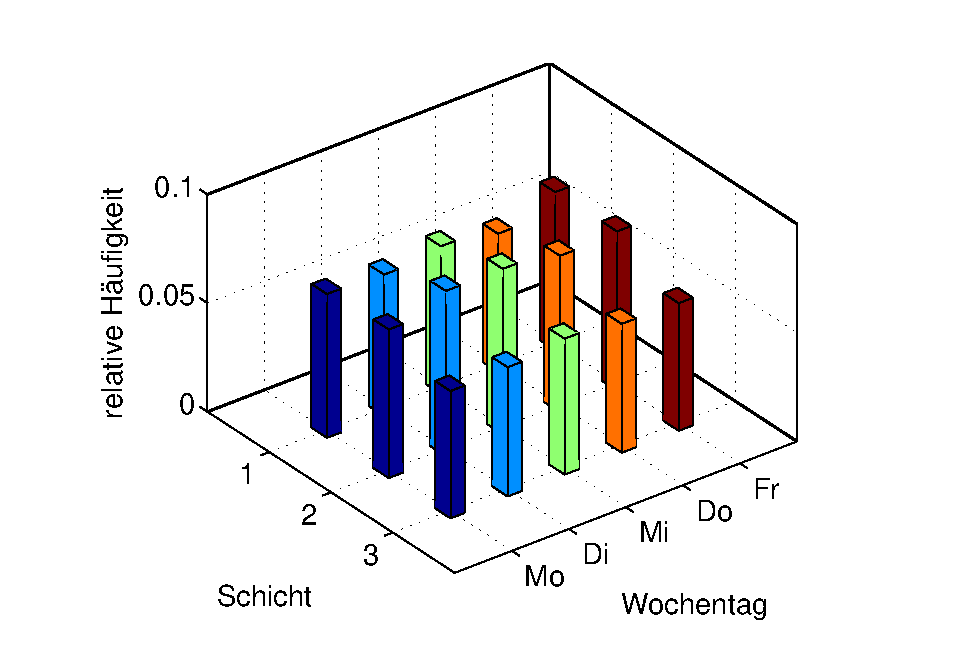
\includegraphics[width=0.5\textwidth]{Kapitel7/Bilder/image1}}
  \caption{Grafische Darstellung der Fertigungsstatistik eines Produktes als relative H\"{a}ufigkeit}
  \label{fig:Fertigungsstatistik1}
\end{figure}

\noindent Das dreidimensionale S\"{a}ulendiagramm wird mit MATLAB mit dem folgenden Programmabschnitt erstellt.

\lstinputlisting[caption = {}]{Kapitel7/mat1.m}

\noindent Ist die Summenh\"{a}ufigkeit einzelner Merkmalsauspr\"{a}gungen interessant, kann der Datensatz als gestapeltes S\"{a}ulendiagramm dargestellt werden. An dieser Darstellung kann direkt abgelesen werden, welche Randh\"{a}ufigkeit sich f\"{u}r eine bestimmte Merkmalsauspr\"{a}gung ergibt. Bild \ref{fig:Fertigungsstatistik2} stellt die absolute Randh\"{a}ufigkeit der Fertigungsschicht dar.

\noindent 
\begin{figure}[H]
  \centerline{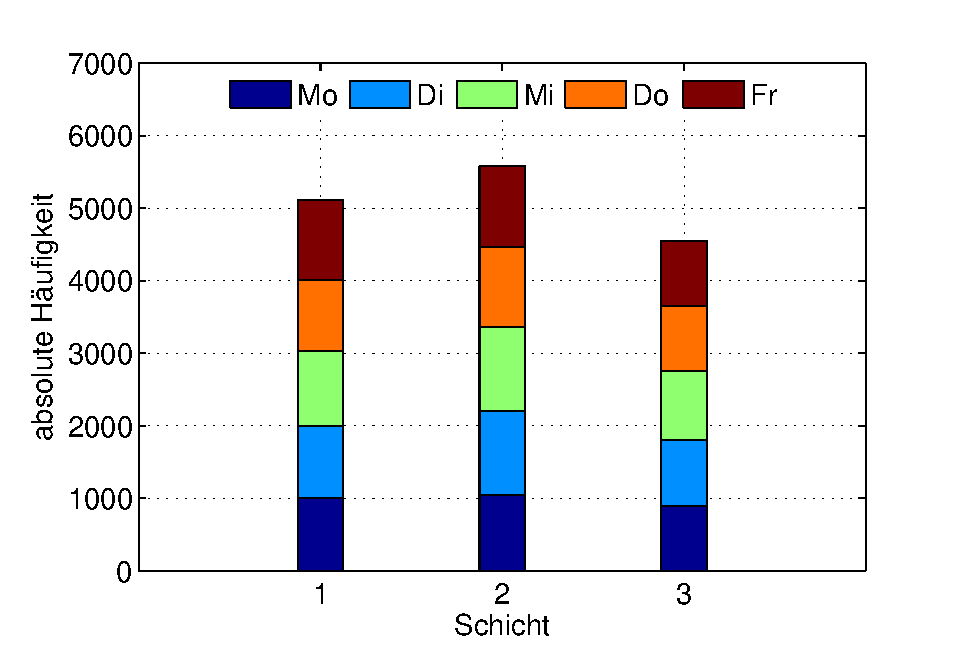
\includegraphics[width=0.5\textwidth]{Kapitel7/Bilder/image2}}
  \caption{Grafische Darstellung der absoluten Randh\"{a}ufigkeit der Fertigungsschicht eines Produktes}
  \label{fig:Fertigungsstatistik2}
\end{figure}

\noindent Die Erzeugung eines gestapelten S\"{a}ulendiagramms mit MATLAB erfolgt in dem folgenden Programmabschnitt.

\lstinputlisting[caption = {}]{Kapitel7/mat2.m}

\noindent Mit dieser Darstellung kann auch der Begriff der bedingten Wahrscheinlichkeit interpretiert werden. Zum Beispiel ergibt sich die relative H\"{a}ufigkeit, mit der ein Produkt am Mittwoch gefertigt wurde, unter der Bedingung, dass es in Schicht 3 gefertigt wurde, aus der relativen Aufteilung der S\"{a}ule Schicht 3. Diese Bedingungen k\"{o}nnen als bedingte Wahrscheinlichkeit aufgefasst werden, die sich berechnen l\"{a}sst als

\begin{equation}\label{eq:sevenseven}
h(x|y)=\dfrac{h(x,y)}{h(x=\text{beliebig},y)} =\dfrac{h(x,y)}{h(y)}
\end{equation}

\noindent mit x = Mi und y = Schicht 3. Die bedingte Wahrscheinlichkeit schr\"{a}nkt die Grundmenge m\"{o}glicher Ereignisse aus y = Schicht 3 ein. Da dabei x beliebig ist, ist die Wahrscheinlichkeit f\"{u}r y = Schicht 3 gerade die Randh\"{a}ufigkeit h(y). F\"{u}r das Beispiel ergibt sich

\begin{equation}\label{eq:seveneight}
h(Mi|3)=\dfrac{0.063}{0.297} =0.2121
\end{equation}

\clearpage

\subsubsection{Zweidimensionale stetige Datens\"{a}tze}

\noindent Auch bei stetigen Gr\"{o}{\ss}en werden die Beobachtungen zun\"{a}chst in einer Urliste dokumentiert. Tabelle 7.6 zeigt ein Beispiel zur Abh\"{a}ngigkeit von Fertigungsdefekten als Funktion der Umgebungstemperatur. Dabei wurde die Anzahl von Fertigungsdefekten an verschiedenen Tagen in Abh\"{a}ngigkeit der Tagestemperatur untersucht.

\begin{table}[H]
\setlength{\arrayrulewidth}{.1em}
\caption{Daten zur Abh\"{a}ngigkeit von Fertigungsdefekten als Funktion der Umgebungstemperatur}
\setlength{\fboxsep}{0pt}%
\colorbox{lightgray}{%
\arrayrulecolor{white}%
\begin{tabular}{ wc{5cm} | wc{1.5cm} | wc{1.5cm} | wc{1.5cm} | wc{1.5cm} | wc{1.5cm} | wc{1.5cm} }
\hline\xrowht{10pt}

\fontfamily{phv}\selectfont\textbf{Tag} &
\fontfamily{phv}\selectfont{1} &
\fontfamily{phv}\selectfont{2} &
\fontfamily{phv}\selectfont{3} &
\fontfamily{phv}\selectfont{4} &
\fontfamily{phv}\selectfont{5} &
\fontfamily{phv}\selectfont{6}\\ \hline \xrowht{10pt}

\fontfamily{phv}\selectfont\textbf{Temperatur T / $\si{\degree}$C} & 
\fontfamily{phv}\selectfont{24.2} &
\fontfamily{phv}\selectfont{22.7} & 
\fontfamily{phv}\selectfont{30.5} &
\fontfamily{phv}\selectfont{28.6} & 
\fontfamily{phv}\selectfont{25.5} &
\fontfamily{phv}\selectfont{32.0} \\ \hline\xrowht{10pt}

\fontfamily{phv}\selectfont\textbf{Anzahl von Defekten D} & 
\fontfamily{phv}\selectfont{25} &
\fontfamily{phv}\selectfont{31} & 
\fontfamily{phv}\selectfont{36} &
\fontfamily{phv}\selectfont{33} & 
\fontfamily{phv}\selectfont{19} &
\fontfamily{phv}\selectfont{24}\\ \hline

\end{tabular}%
}
\label{tab:sevensix}
\end{table}

\begin{table}[H]
\setlength{\arrayrulewidth}{.1em}
\setlength{\fboxsep}{0pt}%
\colorbox{lightgray}{%
\arrayrulecolor{white}%
\begin{tabular}{ wc{5cm} | wc{1.5cm} | wc{1.5cm} | wc{1.5cm} | wc{1.5cm} | wc{1.5cm} | wc{1.5cm} }
\hline\xrowht{10pt}

\fontfamily{phv}\selectfont\textbf{Tag} &
\fontfamily{phv}\selectfont{7} &
\fontfamily{phv}\selectfont{8} &
\fontfamily{phv}\selectfont{9} &
\fontfamily{phv}\selectfont{10} &
\fontfamily{phv}\selectfont{11} &
\fontfamily{phv}\selectfont{12}\\ \hline \xrowht{10pt}

\fontfamily{phv}\selectfont\textbf{Temperatur T / $\si{\degree}$C} & 
\fontfamily{phv}\selectfont{28.6} &
\fontfamily{phv}\selectfont{26.5} & 
\fontfamily{phv}\selectfont{25.3} &
\fontfamily{phv}\selectfont{26.0} & 
\fontfamily{phv}\selectfont{24.4} &
\fontfamily{phv}\selectfont{24.8} \\ \hline\xrowht{10pt}

\fontfamily{phv}\selectfont\textbf{Anzahl von Defekten D} & 
\fontfamily{phv}\selectfont{27} &
\fontfamily{phv}\selectfont{25} & 
\fontfamily{phv}\selectfont{16} &
\fontfamily{phv}\selectfont{14} & 
\fontfamily{phv}\selectfont{22} &
\fontfamily{phv}\selectfont{23}\\ \hline

\end{tabular}%
}
\end{table}

\begin{table}[H]
\setlength{\arrayrulewidth}{.1em}
\setlength{\fboxsep}{0pt}%
\colorbox{lightgray}{%
\arrayrulecolor{white}%
\begin{tabular}{ wc{5cm} | wc{1.5cm} | wc{1.5cm} | wc{1.5cm} | wc{1.5cm} | wc{1.5cm} | wc{1.5cm} }
\hline\xrowht{10pt}

\fontfamily{phv}\selectfont\textbf{Tag} &
\fontfamily{phv}\selectfont{13} &
\fontfamily{phv}\selectfont{14} & 
\fontfamily{phv}\selectfont{15} &
\fontfamily{phv}\selectfont{16} & 
\fontfamily{phv}\selectfont{17} &
\fontfamily{phv}\selectfont{18} \\ \hline \xrowht{10pt}

\fontfamily{phv}\selectfont\textbf{Temperatur T / $\si{\degree}$C} & 
\fontfamily{phv}\selectfont{24.8} &
\fontfamily{phv}\selectfont{20.6} & 
\fontfamily{phv}\selectfont{25.1} &
\fontfamily{phv}\selectfont{21.4} & 
\fontfamily{phv}\selectfont{23.7} &
\fontfamily{phv}\selectfont{25.2} \\ \hline\xrowht{10pt}

\fontfamily{phv}\selectfont\textbf{Anzahl von Defekten D} & 
\fontfamily{phv}\selectfont{20} &
\fontfamily{phv}\selectfont{25} & 
\fontfamily{phv}\selectfont{25} &
\fontfamily{phv}\selectfont{23} & 
\fontfamily{phv}\selectfont{27} &
\fontfamily{phv}\selectfont{30}\\ \hline

\end{tabular}%
}
\end{table}

{\fontfamily{phv}\selectfont
\noindent\textbf{Grafische Darstellung}}\smallskip

\noindent Die Temperatur ist eine stetige Gr\"{o}{\ss}e, es existiert zumindest physikalisch gesehen keine Quantisierung. Bei diesem stetigen Datentyp versagt die Darstellung mit Kontingenztabellen, da unendlich viele Merkmalsauspr\"{a}gungen existieren und die Kontingenztabelle damit unendlich gro{\ss} w\"{u}rde. Eine M\"{o}glichkeit w\"{a}re, die Temperaturdaten zur gruppieren, dann k\"{o}nnte wie in Abschnitt 7.1.1 verfahren werden. Allerdings w\"{u}rden durch die Gruppierung gegebenenfalls wesentliche Informationen verloren gehen.\newline

\noindent Eine zweite M\"{o}glichkeit, den Zusammenhang zwischen Temperatur T und Anzahl von Defekten D aufzuzeigen, ist ein zweidimensionales Streudiagramm, das in Bild \ref{fig:DefekteTemperatur1} dargestellt ist.

\noindent 
\begin{figure}[H]
  \centerline{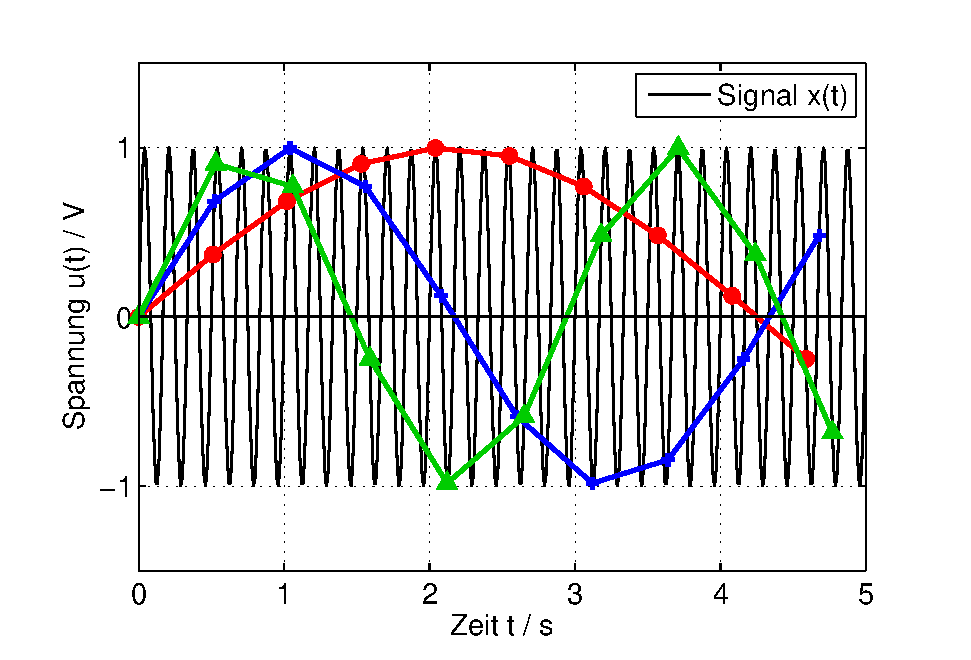
\includegraphics[width=0.5\textwidth]{Kapitel7/Bilder/image3}}
  \caption{Darstellung der Wertepaare aus Tabelle 7.6 in einem Streudiagramm}
  \label{fig:DefekteTemperatur1}
\end{figure}

\noindent Jeder Punkt des Streudiagramms ist ein Datenpunkt der Tabelle. Seine Lage wird durch die beiden Merkmale Temperatur und Anzahl von Defekten festgelegt.

\clearpage

{\fontfamily{phv}\selectfont
\noindent\textbf{Randverteilungen stetiger Datens\"{a}tze}}\smallskip

\noindent Bei der Beschreibung univariater H\"{a}ufigkeiten h(x) wird in Kapitel 3 zur Beschreibung stetiger Daten die Summenh\"{a}ufigkeit H(x) eingef\"{u}hrt. 

\begin{equation}\label{eq:sevennine}
H(x)=\sum _{\xi =-\infty}^{x}h(\xi)
\end{equation}

\noindent Bei stetigen multivariaten Datens\"{a}tzen wird die Summenh\"{a}ufigkeit verwendet, um die Verteilung der Randh\"{a}ufigkeit zu beschreiben. Dabei wird davon ausgegangen, dass alle Variablen bis auf eine Variable beliebig sind. Zum Beispiel ergibt sich f\"{u}r die Randverteilung H(x) eines zweidimensionalen Datensatzes 

\begin{equation}\label{eq:seventen}
H(x)=\sum _{\xi =-\infty}^{x}\sum _{y=-\infty}^{\infty }h(\xi ,y)
\end{equation}

\noindent F\"{u}r die Daten aus Tabelle \ref{tab:sevensix} ergeben sich die in Bild \ref{fig:DefekteTemperatur2} dargestellten Verteilungen der Randh\"{a}ufigkeiten der Temperatur H(T) und der Anzahl von Defekten H(D).

\noindent 
\begin{figure}[H]
  \centerline{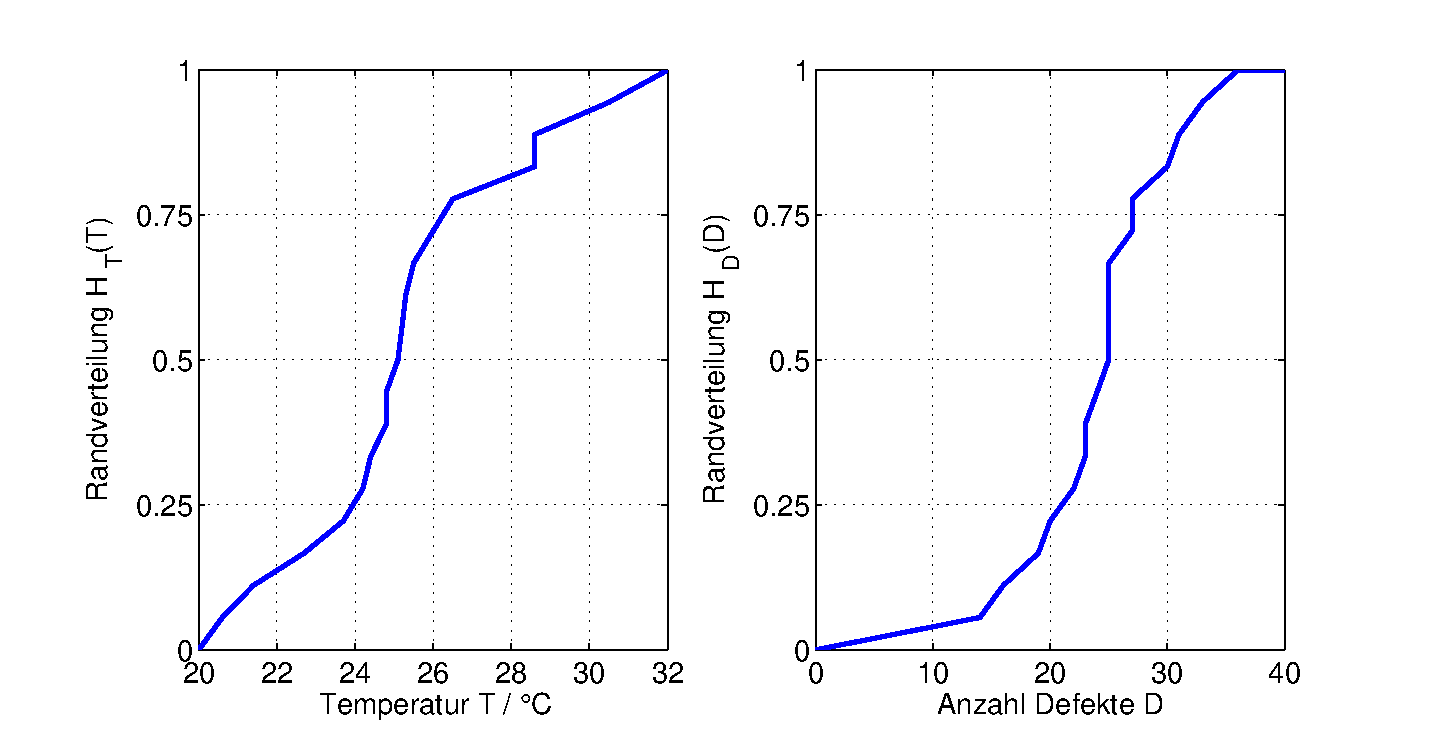
\includegraphics[width=1\textwidth]{Kapitel7/Bilder/image4}}
  \caption{Randverteilungen der Temperatur T und der Anzahl von Defekten D}
  \label{fig:DefekteTemperatur2}
\end{figure}

\noindent Die Randverteilung H(T) beginnt f\"{u}r sehr kleine Temperaturen bei der Wahrscheinlichkeit 0 und endet f\"{u}r sehr gro{\ss}e Werte bei 1, die Aussage gilt sinngem\"{a}{\ss} f\"{u}r die Randverteilung H(D).

\subsubsection{Darstellung und Charakterisierung multivariater Datens\"{a}tze}

\noindent Zweidimensionale Datens\"{a}tze lassen sich wegen der r\"{a}umlichen Vorstellung noch vergleichsweise einfach darstellen. Auch bei dreidimensionalen Datens\"{a}tzen ergeben sich noch M\"{o}glichkeiten der grafischen Darstellung. Dazu wird ein Datensatz analysiert, bei dem die Ausbeute eines chemischen Prozesses als Funktion der Temperatur und der Katalysatorkonzentration dargestellt wird. F\"{u}r die Messwertaufnahme wurden alle anderen Parameter konstant gehalten.\newline

\noindent Soll die Fertigungsausbeute A in Abh\"{a}ngigkeit von Temperatur T und Katalysatorkonzentration K dargestellt werden, kann das in Form eines dreidimensionalen Streudiagramms erfolgen. Dabei wird die r\"{a}umliche Darstellung in die Ebene projiziert.

\clearpage

\begin{table}[H]
\setlength{\arrayrulewidth}{.1em}
\caption{Urliste einer Messreihe eines chemischen Prozesses}
\setlength{\fboxsep}{0pt}%
\colorbox{lightgray}{%
\arrayrulecolor{white}%
\begin{tabular}{ wc{1cm} | wc{4cm} | wc{6cm} | wc{4cm}}
\hline\xrowht{10pt}

\fontfamily{phv}\selectfont\textbf{Nr.} &
\fontfamily{phv}\selectfont\textbf{Temperatur T / $\si{\degree}$C} &
\fontfamily{phv}\selectfont\textbf{Katalysatorkonzentration K / \%} &
\fontfamily{phv}\selectfont\textbf{Ausbeute A / \%}\\ \hline \xrowht{10pt}

\fontfamily{phv}\selectfont{1} & 
\fontfamily{phv}\selectfont{130} &
\fontfamily{phv}\selectfont{0.3} & 
\fontfamily{phv}\selectfont{67.47} \\ \hline\xrowht{10pt}

\fontfamily{phv}\selectfont{2} & 
\fontfamily{phv}\selectfont{140} &
\fontfamily{phv}\selectfont{0.5} & 
\fontfamily{phv}\selectfont{84.27}\\ \hline\xrowht{10pt}

\fontfamily{phv}\selectfont{3} & 
\fontfamily{phv}\selectfont{120} &
\fontfamily{phv}\selectfont{0.1} & 
\fontfamily{phv}\selectfont{54.78}\\ \hline\xrowht{10pt}

\fontfamily{phv}\selectfont{4} & 
\fontfamily{phv}\selectfont{120} &
\fontfamily{phv}\selectfont{0.1} & 
\fontfamily{phv}\selectfont{54.13}\\ \hline\xrowht{10pt}

\fontfamily{phv}\selectfont{5} & 
\fontfamily{phv}\selectfont{120} &
\fontfamily{phv}\selectfont{0.5} & 
\fontfamily{phv}\selectfont{73.82}\\ \hline\xrowht{10pt}

\fontfamily{phv}\selectfont{6} & 
\fontfamily{phv}\selectfont{130} &
\fontfamily{phv}\selectfont{0.3} & 
\fontfamily{phv}\selectfont{66.18}\\ \hline\xrowht{10pt}

\fontfamily{phv}\selectfont{7} & 
\fontfamily{phv}\selectfont{140} &
\fontfamily{phv}\selectfont{0.5} & 
\fontfamily{phv}\selectfont{83.05}\\ \hline\xrowht{10pt}

\fontfamily{phv}\selectfont{8} & 
\fontfamily{phv}\selectfont{140} &
\fontfamily{phv}\selectfont{0.1} & 
\fontfamily{phv}\selectfont{61.86}\\ \hline\xrowht{10pt}

\fontfamily{phv}\selectfont{9} & 
\fontfamily{phv}\selectfont{140} &
\fontfamily{phv}\selectfont{0.1} & 
\fontfamily{phv}\selectfont{61.33}\\ \hline\xrowht{10pt}

\fontfamily{phv}\selectfont{10} & 
\fontfamily{phv}\selectfont{120} &
\fontfamily{phv}\selectfont{0.5} & 
\fontfamily{phv}\selectfont{71.20} \\ \hline\xrowht{10pt}

\fontfamily{phv}\selectfont{11} & 
\fontfamily{phv}\selectfont{140} &
\fontfamily{phv}\selectfont{0.1} & 
\fontfamily{phv}\selectfont{60.41}\\ \hline\xrowht{10pt}

\fontfamily{phv}\selectfont{12} & 
\fontfamily{phv}\selectfont{130} &
\fontfamily{phv}\selectfont{0.3} & 
\fontfamily{phv}\selectfont{69.08}\\ \hline\xrowht{10pt}

\fontfamily{phv}\selectfont{13} & 
\fontfamily{phv}\selectfont{120} &
\fontfamily{phv}\selectfont{0.1} & 
\fontfamily{phv}\selectfont{51.06}\\ \hline\xrowht{10pt}

\fontfamily{phv}\selectfont{14} & 
\fontfamily{phv}\selectfont{120} &
\fontfamily{phv}\selectfont{0.5} & 
\fontfamily{phv}\selectfont{84.95}\\ \hline\xrowht{10pt}

\fontfamily{phv}\selectfont{15} & 
\fontfamily{phv}\selectfont{120} &
\fontfamily{phv}\selectfont{0.5} & 
\fontfamily{phv}\selectfont{71.31}\\ \hline\xrowht{10pt}

\fontfamily{phv}\selectfont{16} & 
\fontfamily{phv}\selectfont{120} &
\fontfamily{phv}\selectfont{0.1} & 
\fontfamily{phv}\selectfont{53.67}\\ \hline\xrowht{10pt}

\fontfamily{phv}\selectfont{17} & 
\fontfamily{phv}\selectfont{140} &
\fontfamily{phv}\selectfont{0.5} & 
\fontfamily{phv}\selectfont{83.50}\\ \hline\xrowht{10pt}

\fontfamily{phv}\selectfont{18} & 
\fontfamily{phv}\selectfont{120} &
\fontfamily{phv}\selectfont{0.5} & 
\fontfamily{phv}\selectfont{71.87}\\ \hline\xrowht{10pt}

\fontfamily{phv}\selectfont{19} & 
\fontfamily{phv}\selectfont{140} &
\fontfamily{phv}\selectfont{0.1} & 
\fontfamily{phv}\selectfont{61.78}\\ \hline\xrowht{10pt}

\fontfamily{phv}\selectfont{20} & 
\fontfamily{phv}\selectfont{130} &
\fontfamily{phv}\selectfont{0.3} & 
\fontfamily{phv}\selectfont{66.23}\\ \hline

\end{tabular}%
}
\label{tab:sevenseven}
\end{table}

\noindent Bild \ref{fig:ChemischeIndustrie1} stellt die Ausbeute A in Abh\"{a}ngigkeit der Temperatur T und Katalysatorkonzentration K als Streudiagramm dar.

\noindent 
\begin{figure}[H]
  \centerline{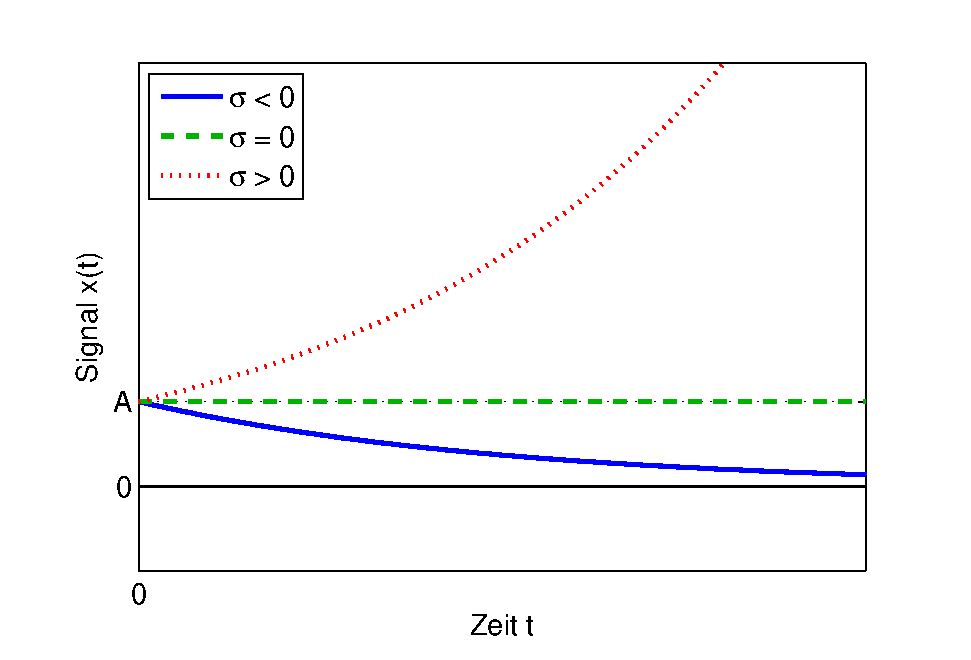
\includegraphics[width=0.5\textwidth]{Kapitel7/Bilder/image5}}
  \caption{Ausbeute in Abh\"{a}ngigkeit der Temperatur und der Katalysatorkonzentration als Streudiagramm}
  \label{fig:ChemischeIndustrie1}
\end{figure}

\clearpage 

\noindent Ein dreidimensionales Streudiagramm mit MATLAB wird \"{u}ber den folgenden Programmabschnitt erstellt.

\lstinputlisting[caption = {}]{Kapitel7/mat3.m}

\noindent Bereits die Darstellung von dreidimensionalen Datens\"{a}tzen f\"{u}hrt zu Messpunkten im Streudiagramm, deren Lagen wegen der Projektion nicht mehr eindeutig erkennbar sind. Steigt die Dimension des Datensatzes auf einen Wert gr\"{o}{\ss}er drei, ist auch eine quasi-r\"{a}umliche Darstellung der Daten nicht mehr m\"{o}glich, sodass hier andere Wege der grafischen Darstellung gefunden werden m\"{u}ssen. \newline

\noindent Eine einfache Darstellungsm\"{o}glichkeit mehrdimensionaler Datens\"{a}tze besteht darin, jeweils f\"{u}r zwei Gr\"{o}{\ss}en ein Streudiagramm zu bilden. Es ergibt sich eine Matrix von Streudiagrammen, bei der der Zusammenhang zwischen zwei Gr\"{o}{\ss}en dargestellt ist. Alle \"{u}brigen Gr\"{o}{\ss}en werden nicht eingeschr\"{a}nkt, sind also beliebig. Auf der Hauptdiagonalen der Matrix sind die Gr\"{o}{\ss}en bezeichnet und die verwendeten Einheiten sind dargestellt. Die Achsenbeschriftung befindet sich jeweils am Rand der Matrix.

\noindent 
\begin{figure}[H]
  \centerline{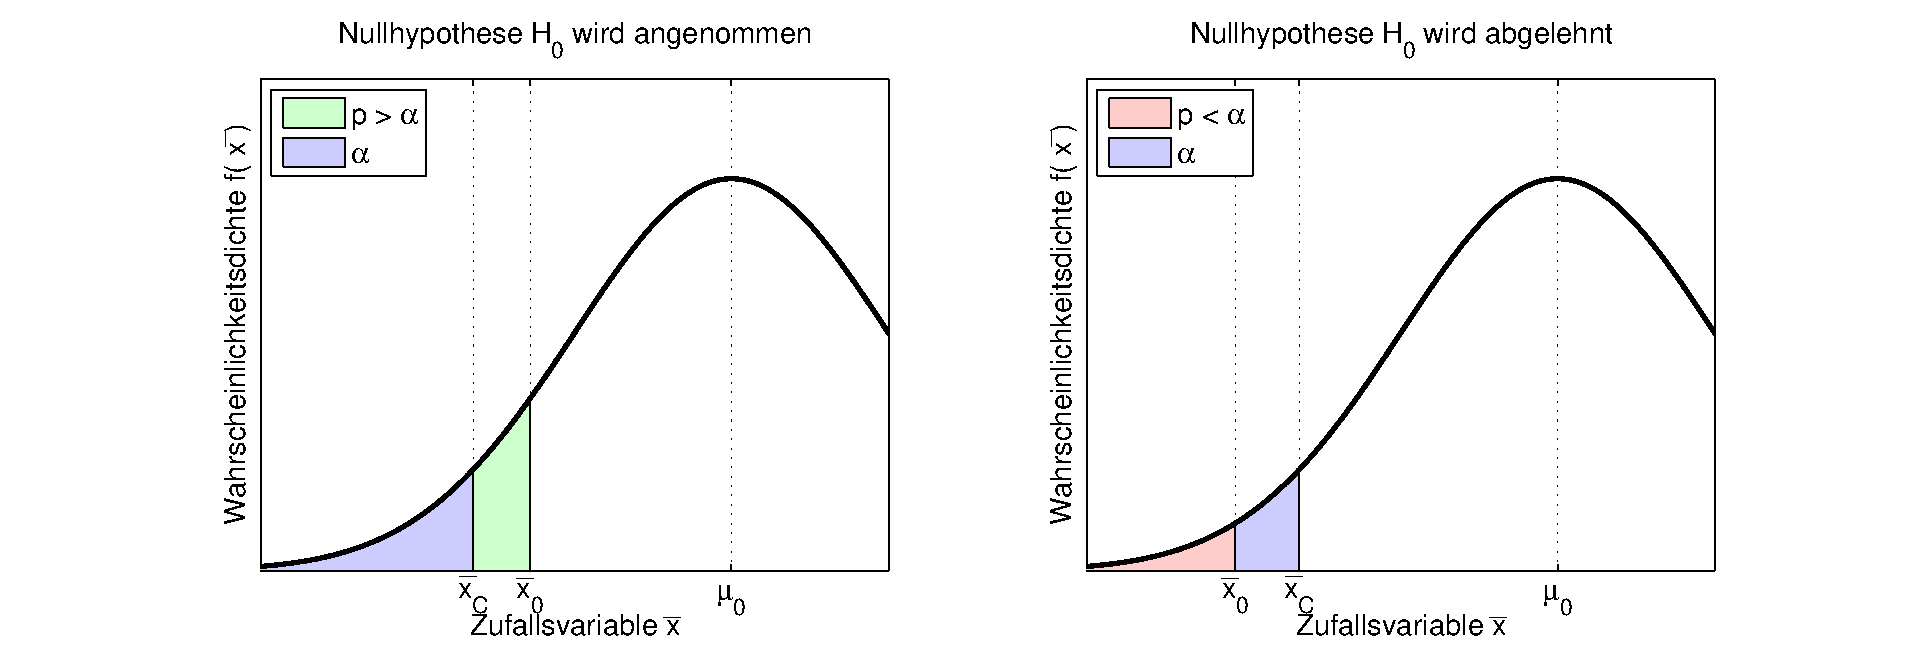
\includegraphics[width=1\textwidth]{Kapitel7/Bilder/image6}}
  \caption{Streudiagramm-Matrix der Messwerte eines chemischen Prozesses}
  \label{fig:ChemischeIndustrie2}
\end{figure}

\noindent Bild \ref{fig:ChemischeIndustrie2} stellt die Streudiagramm-Matrix der Messwerte eines chemischen Prozesses mit den Werten aus Tabelle \ref{tab:sevenseven} dar. Die Matrix ist symmetrisch zur Hauptdiagonalen. An der grafischen Darstellung kann abgelesen werden, welche Kombinationen von Temperatur und Katalysatorkonzentration verwendet wurden. Es wird au{\ss}erdem deutlich, dass die Ausbeute von der Temperatur und der Katalysatorkonzentration abh\"{a}ngig ist. Sowohl eine Erh\"{o}hung der Temperatur als auch der Katalysatorkonzentration k\"{o}nnte in dem untersuchten Parameterbereich somit zur Steigerung der Ausbeute verwendet werden.\newline

\noindent Diese Art der Darstellung kann durch die relative H\"{a}ufigkeitsverteilung der einzelnen Stichprobengr\"{o}{\ss}en erweitert werden. Die H\"{a}ufigkeitsverteilungen werden auf der Hauptdiagonale platziert. Dadurch werden in dem Diagramm mehr Informationen dargestellt, allerdings wirkt die Darstellung weniger \"{u}bersichtlich und die Zuordnung der Daten zu den Gr\"{o}{\ss}en ist weniger deutlich. Bild \ref{fig:ChemischeIndustrie3} stellt diese Variante der Streudiagramm-Matrix dar.

\noindent 
\begin{figure}[H]
  \centerline{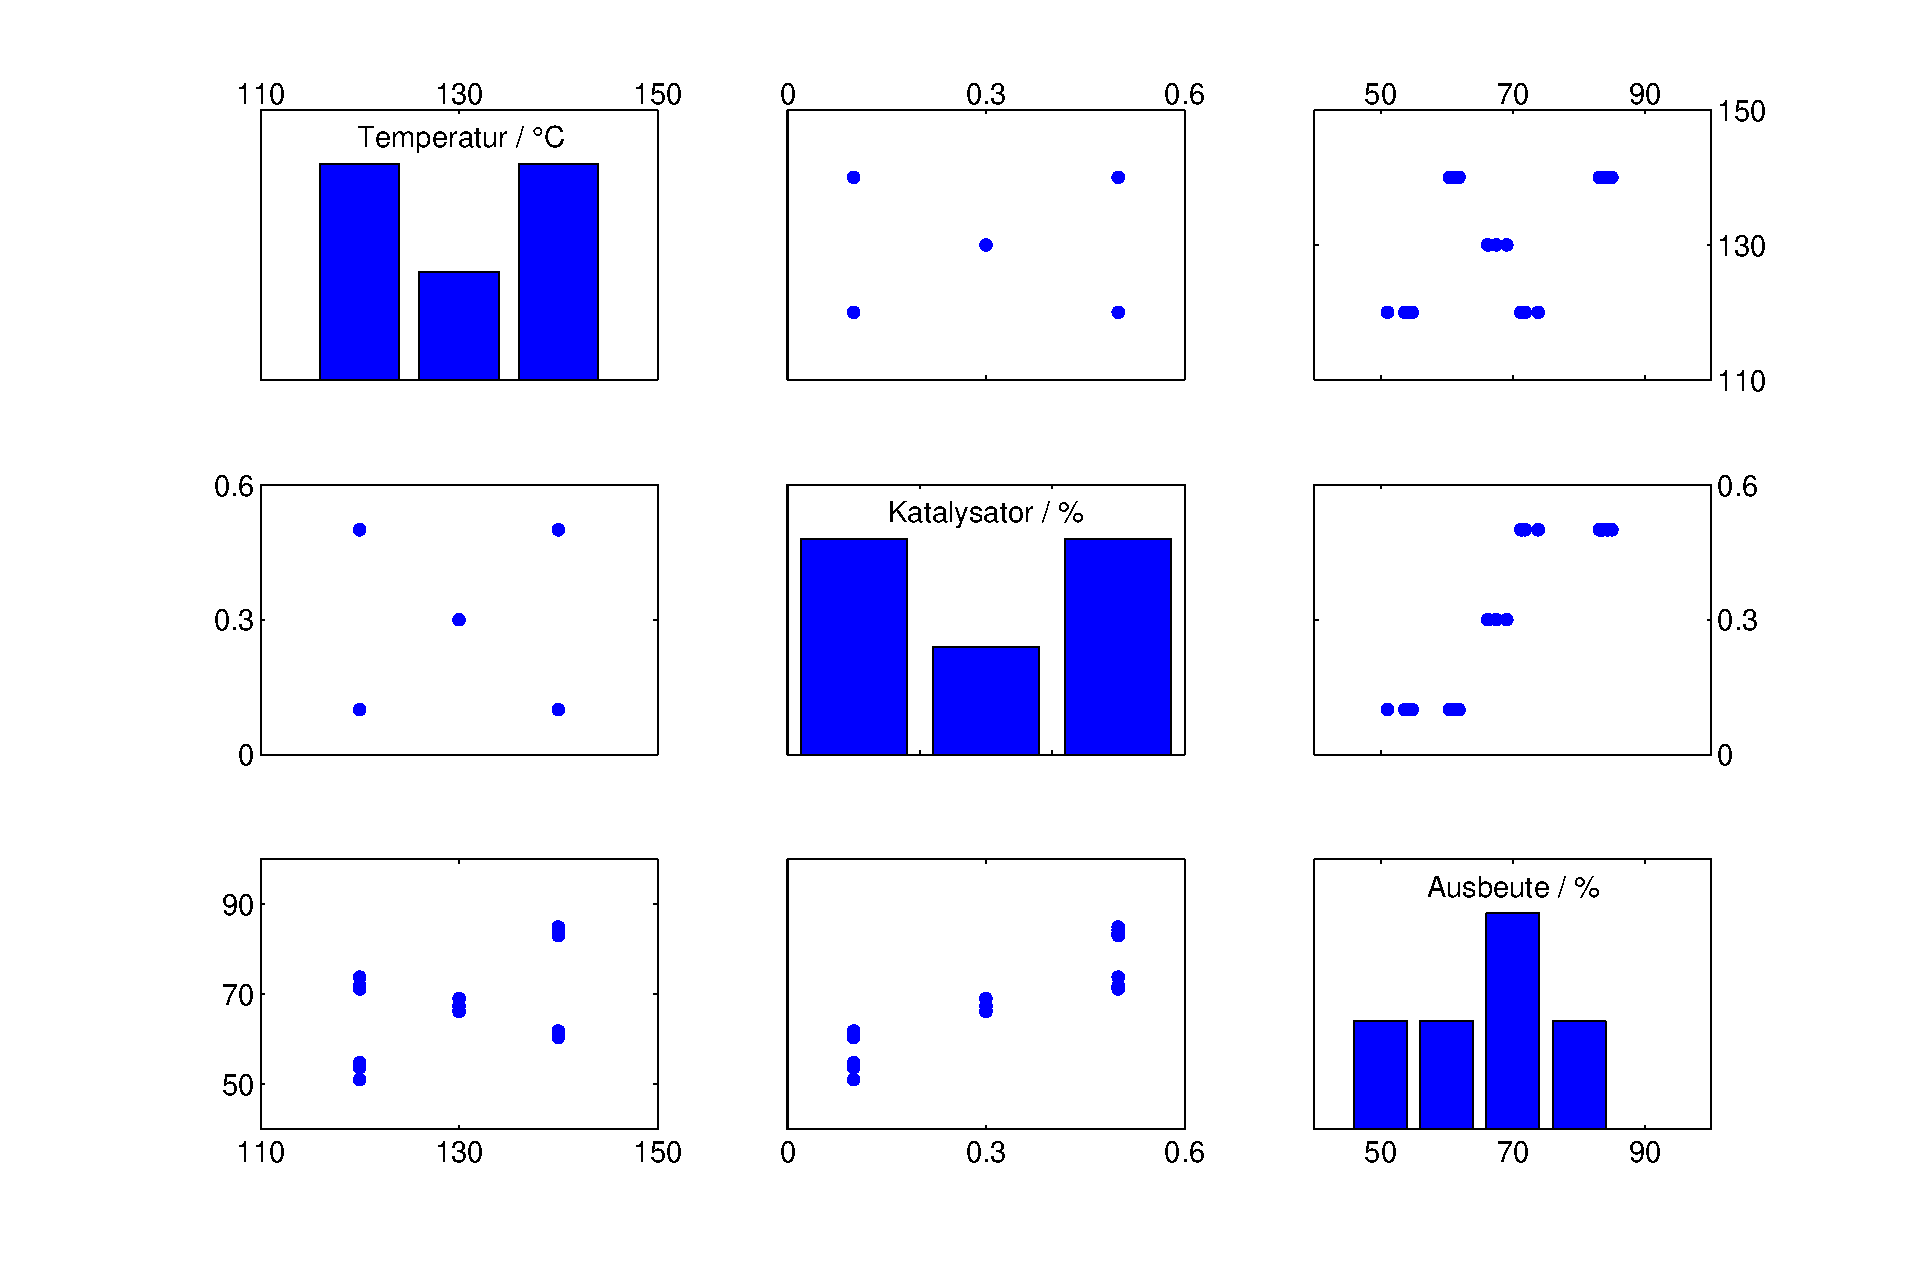
\includegraphics[width=1\textwidth]{Kapitel7/Bilder/image7}}
  \caption{Streudiagramm-Matrix der Messwerte eines chemischen Prozessesmit H\"{a}ufigkeitsverteilung der Stichprobengr\"{o}{\ss}en}
  \label{fig:ChemischeIndustrie3}
\end{figure}

\noindent Die paarweise Streudiagramm-Matrix kann f\"{u}r m-dimensionale Stichproben entsprechend erweitert werden. In MATLAB k\"{o}nnen sie durch Anwendung eines sogenannten subplot realisiert werden. Alternativ kann die Streudiagramm-Matrix mit dem MATLAB-Befehl gplotmatrix dargestellt werden. 

\lstinputlisting[caption = {}]{Kapitel7/mat4.m}

\clearpage

\subsubsection{MATLAB- und Python-Befehle Darstellung multivariater Datens\"{a}tze}

\noindent Der Vollst\"{a}ndigkeit halber sind in Tabelle \ref{tab:seveneight} MATLAB-Befehle zur Darstellung multivariater Datens\"{a}tze zusammengefasst.

\begin{table}[H]
\setlength{\arrayrulewidth}{.1em}
\caption{Zusammenfassung von MATLAB-Befehlen zur Darstellung multivariater Datens\"{a}tze}
\setlength{\fboxsep}{0pt}%
\colorbox{lightgray}{%
\arrayrulecolor{white}%
\begin{tabular}{ wc{8.3cm} | wc{8.3cm} }
\hline\xrowht{10pt}

\fontfamily{phv}\selectfont\textbf{MATLAB-Befehl} &
\fontfamily{phv}\selectfont\textbf{Funktionsbeschreibung} \\ \hline \xrowht{10pt}

\multirow{2}{*}{\fontfamily{phv}\selectfont{bar3(X)}} &
\fontfamily{phv}\selectfont{Darstellung eines dreidimensionalen Datensatzes} \\
& \fontfamily{phv}\selectfont{als räumliches Balkendiagramm}\\ \hline\xrowht{10pt}

\multirow{2}{*}{\fontfamily{phv}\selectfont{scatter3(X)}} &
\fontfamily{phv}\selectfont{Darstellung eines dreidimensionalen Datensatzes} \\
& \fontfamily{phv}\selectfont{als räumliches Streudiagramm}\\ \hline\xrowht{10pt}

\multirow{2}{*}{\fontfamily{phv}\selectfont{gplotmatrix(X)}} &
\fontfamily{phv}\selectfont{Darstellung eStreudiagramm-Matrix f\"{u}r} \\
& \fontfamily{phv}\selectfont{die Daten X}\\ \hline

\end{tabular}%
}
\label{tab:seveneight}
\end{table}

\noindent In  erreicht, der eigentliche Befehl f\"{u}r ein Balkendiagramm oder ein Streudiagramm ist identisch zu der zweidimensionalen Darstellung. Der Befehl gplotmatrix ist in der Bibliothek pandas.plotting verf\"{u}gbar. Alternativ k\"{o}nnen diese Grafiken \"{u}ber eine Matrix von Diagrammen erzeugt werden.Tabelle \ref{tab:sevennine} sind die entsprechenden Python-Befehle aus der Bibliothek matplotlib.pyplot zur Darstellung multivariater Datens\"{a}tze zusammengefasst. Dabei wird die r\"{a}umliche Darstellung \"{u}ber den Parameter projection = '3d' erreicht, der eigentliche Befehl f\"{u}r ein Balkendiagramm oder ein Streudiagramm ist identisch zu der zweidimensionalen Darstellung. Der Befehl gplotmatrix ist in der Bibliothek pandas.plotting verf\"{u}gbar. Alternativ k\"{o}nnen diese Grafiken \"{u}ber eine Matrix von Diagrammen erzeugt werden.

\begin{table}[H]
\setlength{\arrayrulewidth}{.1em}
\caption{Zusammenfassung von Python-Befehlen zur Darstellung multivariater Datens\"{a}tze}
\setlength{\fboxsep}{0pt}%
\colorbox{lightgray}{%
\arrayrulecolor{white}%
\begin{tabular}{ wc{8.3cm} | wc{8.3cm} }
\hline\xrowht{10pt}

\fontfamily{phv}\selectfont\textbf{Python-Befehl} &
\fontfamily{phv}\selectfont\textbf{Funktionsbeschreibung} \\ \hline \xrowht{10pt}

\multirow{2}{*}{\fontfamily{phv}\selectfont{bar(X)}} &
\fontfamily{phv}\selectfont{Darstellung eines dreidimensionalen Datensatzes} \\
& \fontfamily{phv}\selectfont{als räumliches Balkendiagramm}\\ \hline\xrowht{10pt}

\multirow{2}{*}{\fontfamily{phv}\selectfont{scatter(X)}} &
\fontfamily{phv}\selectfont{Darstellung eines dreidimensionalen Datensatzes} \\
& \fontfamily{phv}\selectfont{als räumliches Streudiagramm}\\ \hline\xrowht{10pt}

\multirow{2}{*}{\fontfamily{phv}\selectfont{scatter\_matrix(X)}} &
\fontfamily{phv}\selectfont{Darstellung eStreudiagramm-Matrix f\"{u}r} \\
& \fontfamily{phv}\selectfont{die Daten X}\\ \hline

\end{tabular}%
}
\label{tab:sevennine}
\end{table}

\clearpage

\subsection{Kenngr\"{o}{\ss}en multivariater Stichproben}

\noindent Wie bei univariaten Stichproben k\"{o}nnen multivariate Datens\"{a}tze durch Kenngr\"{o}{\ss}en zusammenfassend beschrieben werden. Dabei wird analog zu der univariaten Berechnung vorgegangen. Im Folgenden wird der arithmetische Mittelwert als Lagekenngr\"{o}{\ss}e vorgestellt. Die Streuung der Gr\"{o}{\ss}en und die Abh\"{a}ngigkeiten der einzelnen Gr\"{o}{\ss}en untereinander werden mit der Kovarianz oder der Korrelation gekennzeichnet. 

\subsubsection{Arithmetischer Mittelwertsvektor einer Stichprobe}

\noindent In Kapitel 3 wird der arithmetische Mittelwert einer univariaten Stichprobe x$_{1}$, ..., x$_{N}$ definiert zu

\begin{equation}\label{eq:seveneleven}
\bar{x}=\dfrac{x_{1} + ... +x_{N} }{N} =\dfrac{1}{N} \cdot \sum _{n=1}^{N}x_{n}
\end{equation}

\noindent F\"{u}r die Beschreibung einer M-dimensionalen Stichprobe mit M eindimensionalen Zufallsvariablen $\underbar{x}_{1}, \dots, \underbar{x}_{M}$ wird die Vektorschreibweise angewendet. Die Matrix \textbf{X} aller Messwerte ergibt sich aus den N Messwerten jeder Gr\"{o}{\ss}e.

\begin{equation}\label{eq:seventwelve}
X=\left(\begin{array}{ccc} {\underline{x}_{1} } & {\cdots } & {\underline{x}_{M} } \end{array}\right)=\left(\begin{array}{cccc} {x_{11} } & {x_{12} } & {\cdots } & {x_{1M}} \\ 
{x_{21} } & {x_{22} } & {\cdots } & {x_{2M}} \\ 
{\vdots } & {\vdots } & {} & {\vdots } \\ 
{x_{N1} } & {x_{N2} } & {\cdots } & {x_{NM}} \end{array}\right)
\end{equation}

\noindent Der arithmetische Mittelwert einer M-dimensionalen Stichprobe wird damit auf die Berechnung M einzelner Mittelwerte zur\"{u}ckgef\"{u}hrt.

\begin{equation}\label{eq:seventhirteen}
\underline{\bar{x}}^{T} =\left(\begin{array}{ccc} {\bar{x}_{1}} & {\cdots} & {\bar{x}_{M}} \end{array}\right)=\left(\begin{array}{ccc} {\dfrac{1}{N} \cdot \sum _{n=1}^{N}x_{n1}} & {\cdots} & {\dfrac{1}{N} \cdot \sum _{n=1}^{N}x_{nM}} \end{array}\right)
\end{equation}

\noindent F\"{u}r die Stichprobe eines chemischen Prozesses aus Tabelle \ref{tab:sevenseven} ergibt sich ein Vektor der Mittelwerte von

\begin{equation}\label{eq:sevenfourteen}
\bar{\underline{x}}^{T} =\left(\begin{array}{ccc} {130.00} & {0.30} & {67.60} \end{array}\right)
\end{equation}

\noindent In MATLAB wird der Mittelwertsvektor der Messreihe mit folgender Befehlssequenz berechnet:

\lstinputlisting[caption = {}]{Kapitel7/mat5.m}

\noindent Bei einer mittleren Temperatur von 130 $\si{\degree}$C und einer mittleren Katalysatorkonzentration von 0.3 \% ist eine Ausbeute von 67.6 \% zu erwarten.

\clearpage

\subsubsection{Kovarianzmatrix einer Stichprobe}

\noindent Um einen Zusammenhang mehrerer Zufallsvariablen quantitativ zu beschreiben, kann auf Basis der vorliegenden Stichprobe die Kovarianz berechnet werden. Zum besseren Verst\"{a}ndnis und aus Gr\"{u}nden der Darstellung wird zun\"{a}chst wieder die Kovarianz f\"{u}r eine zweidimensionale Stichprobe eingef\"{u}hrt. Die dabei gewonnenen Erkenntnisse werden dann auf mehrdimensionale Stichproben erweitern.

{\fontfamily{phv}\selectfont
\noindent\textbf{Kovarianz einer zweidimensionalen Stichprobe}}\smallskip

\noindent Die zweidimensionale Stichrobe besteht aus N Wertepaaren der Form 

\begin{equation}\label{eq:sevenfifteen}
\left(\begin{array}{cc} {\underline{x}} & {\underline{y}} \end{array}\right)=\left(\begin{array}{cc} {x_{1} } & {y_{1} } \\ {\vdots } & {\vdots } \\ {x_{N} } & {y_{N} } \end{array}\right)
\end{equation}

\noindent Um eine Kennzahl zu berechnen, die den Zusammenhang zwischen den einzelnen Datenpaaren angibt, werden zun\"{a}chst die jeweiligen Mittelwerte der x-Werte der Stichprobe 

\begin{equation}\label{eq:sevensixteen}
\bar{x}=\dfrac{1}{N} \cdot \left(x_{1} +x_{2} +...+x_{N} \right)=\dfrac{1}{N} \cdot \sum _{n=1}^{N}x_{n}
\end{equation}

\noindent und der y-Werte der Stichprobe 

\begin{equation}\label{eq:sevenseventeen}
\bar{y}=\dfrac{1}{N} \cdot \left(y_{1} +y_{2} +...+y_{N} \right)=\dfrac{1}{N} \cdot \sum _{n=1}^{N}y_{n}
\end{equation}

\noindent berechnet. F\"{u}r das Datenpaar mit dem Index n ist damit die Abweichung vom Mittelwert gegeben durch 

\begin{equation}\label{eq:seveneighteen}
\Delta x_{n} =x_{n} -\bar{x}
\end{equation}

\noindent beziehungsweise

\begin{equation}\label{eq:sevennineteen}
\Delta y_{n} =y_{n} -\bar{y}
\end{equation}

\clearpage

\noindent Damit wird der zugrunde liegende Datensatz zentriert, was in Bild \ref{fig:DefekteTemperatur3} verdeutlicht wird.

\noindent 
\begin{figure}[H]
  \centerline{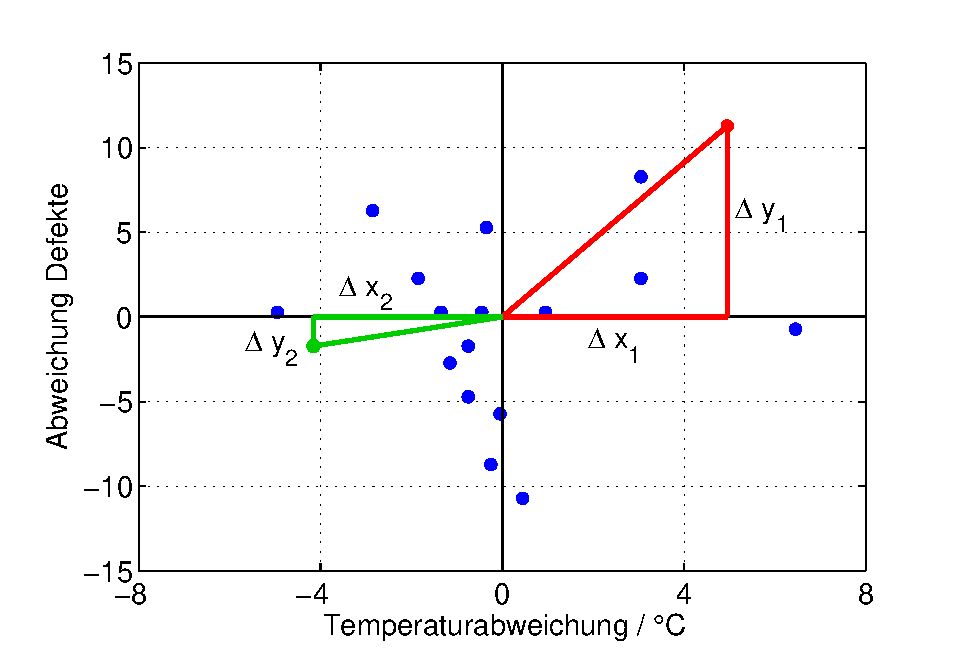
\includegraphics[width=0.5\textwidth]{Kapitel7/Bilder/image8}}
  \caption{Darstellung der Abweichung der Wertepaare aus Tabelle \ref{tab:sevensix} von ihrem jeweiligen Mittelwert in einem Streudiagramm}
  \label{fig:DefekteTemperatur3}
\end{figure}

\noindent F\"{u}r gro{\ss}e Werte von x$_{n}$ ist $\Delta$x$_{n}$ positiv, w\"{a}hrend $\Delta$x$_{n}$ f\"{u}r kleine Werte von x$_{n}$ negativ ist. Diese Aussagen gelten f\"{u}r die Werte von y$_{n}$ entsprechend. Wenn also gro{\ss}e x-Werte gew\"{o}hnlich mit gro{\ss}en y-Werten und kleine x-Werte gew\"{o}hnlich mit kleinen y-Werten auftreten, dann sind die Vorzeichen von $\Delta$x$_{n}$ und $\Delta$y$_{n}$ gleich. Damit wird aber das Produkt der Abweichungen vom Mittelwert gr\"{o}{\ss}er als null.

\begin{equation}\label{eq:seventwenty}
\Delta y_{n} =y_{n} -\bar{y}
\end{equation}

\noindent F\"{u}r diesen Fall wird auch die Summe aller Produkte

\begin{equation}\label{eq:seventwentyone}
\sum _{n=1}^{N}\left((x_{n} -\bar{x})\cdot (y_{n} -\bar{y})\right) >0
\end{equation}

\noindent gr\"{o}{\ss}er als null sein. Liegen bei einer Stichprobe gro{\ss}e x-Werte gew\"{o}hnlich mit kleinen y-Werten und kleine x-Werte mit gro{\ss}en y-Werten zusammen, dann sind die Vorzeichen von $\Delta$x$_{n}$ und $\Delta$y$_{n}$ gew\"{o}hnlich unterschiedlich. Damit wird das Produkt der Abweichung vom Mittelwert kleiner null sein. Entsprechendes gilt f\"{u}r deren Summe. Je gr\"{o}{\ss}er der Betrag der Summe ist, desto klarer ist die Aussage eines linearen Zusammenhangs der Zufallsgr\"{o}{\ss}en x und y.

\noindent Aus der Summe aller Produkte in Gleichung \eqref{eq:seventwentyone} ergibt sich durch die Normierung mit N - 1 die Kovarianz der Gr\"{o}{\ss}en x und y.

\begin{equation}\label{eq:seventwentytwo}
s_{xy} =\dfrac{1}{N-1} \cdot \sum _{n=1}^{N}\left((x_{n} -\bar{x})\cdot (y_{n} -\bar{y})\right) 
\end{equation}

\noindent Der Wert der Kovarianz ist entsprechend den obigen \"{U}berlegungen positiv, wenn x und y tendenziell einen gleichsinnigen linearen Zusammenhang aufweisen. Dagegen ist die Kovarianz negativ, wenn x und y einen gegensinnig linearen Zusammenhang besitzen. Bei einer Kovarianz von s$_{xy}$ = 0 sind die Gr\"{o}{\ss}en x und y voneinander unabh\"{a}ngig. \bigskip

{\fontfamily{phv}\selectfont
\noindent\textbf{Kovarianzmatrix einer multivariaten Stichprobe}}\smallskip

\noindent Durch die Darstellung multivariater Gr\"{o}{\ss}en in Streudiagramm-Matrizen wird die mehrdimensionale Darstellung in eine zweidimensionale Darstellung transformiert. Ganz analog wird bei der Kovarianz verfahren. Es ergibt sich die Kovarianzmatrix \textbf{S}.

\begin{equation}\label{eq:seventwentythree}
\begin{split}
S & = \left(\begin{array}{ccc} {s_{1}^{2} } & {\ldots } & {s_{1M}^{} } \\ {\vdots } & {\ddots } & {\vdots } \\ {s_{M1}^{} } & {\cdots } & {s_{M}^{2} } \end{array}\right) \\ 
& = \left(\begin{array}{ccc} {\dfrac{1}{N-1} \cdot \sum\limits _{n=1}^{N}\left(x_{n1} -\bar{x}_{1} \right)^{2}  } & {\ldots } & {\dfrac{1}{N-1} \cdot \sum\limits _{n=1}^{N}\left(x_{n1} -\bar{x}_{1} \right)\cdot \left(x_{nM} -\bar{x}_{M} \right) } \\ {\vdots } & {} & {\vdots } \\ {\dfrac{1}{N-1} \cdot \sum\limits _{n=1}^{N}\left(x_{nM} -\bar{x}_{M} \right)\cdot \left(x_{n1} -\bar{x}_{1} \right) } & {\cdots } & {\dfrac{1}{N-1} \cdot \sum\limits _{n=1}^{N}\left(x_{nM} -\bar{x}_{M} \right)^{2}} \end{array}\right)
\end{split}
\end{equation}

\noindent Gleichung \eqref{eq:seventwentythree} kann in Vektorschreibweise \"{u}berf\"{u}hrt werden. Mit der Matrix \textbf{X} von Stichprobenwerten

\begin{equation}\label{eq:seventwentyfour}
X=\left(\begin{array}{ccc} {\underline{x}_{1} } & {\cdots } & {\underline{x}_{M} } \end{array}\right)=\left(\begin{array}{cccc} {x_{11} } & {x_{12} } & {\cdots } & {x_{1M} } \\ {x_{21} } & {x_{22} } & {\cdots } & {x_{2M} } \\ {\vdots } & {\vdots } & {} & {\vdots } \\ {x_{N1} } & {x_{N2} } & {\cdots } & {x_{NM} } \end{array}\right)
\end{equation}

\noindent und dem Vektor der Mittelwerte 

\begin{equation}\label{eq:seventwentyfive}
\underline{\bar{x}}^{T} =\left(\begin{array}{ccc} {\bar{x}_{1} } & {\cdots } & {\bar{x}_{M} } \end{array}\right)=\left(\begin{array}{ccc} {\dfrac{1}{N} \cdot \sum\limits _{n=1}^{N}x_{n1}  } & {\cdots } & {\dfrac{1}{N} \cdot \sum\limits _{n=1}^{N}x_{nM}  } \end{array}\right)
\end{equation}

\noindent kann Gleichung \eqref{eq:seventwentythree} umgeschrieben werden zu

\begin{equation}\label{eq:seventwentysix}
\begin{split}
S & = \left(\begin{array}{ccc} {\dfrac{1}{N-1} \cdot \sum\limits _{n=1}^{N}\left(x_{n1} -\bar{x}_{1} \right)^{2}  } & {\ldots } & {\dfrac{1}{N-1} \cdot \sum\limits _{n=1}^{N}\left(x_{n1} -\bar{x}_{1} \right)\cdot \left(x_{nM} -\bar{x}_{M} \right) } \\ {\vdots } & {} & {\vdots } \\ {\dfrac{1}{N-1} \cdot \sum\limits _{n=1}^{N}\left(x_{nM} -\bar{x}_{M} \right)\cdot \left(x_{n1} -\bar{x}_{1} \right) } & {\cdots } & {\dfrac{1}{N-1} \cdot \sum\limits _{n=1}^{N}\left(x_{nM} -\bar{x}_{M} \right)^{2}  } \end{array}\right) \\ 
& = \dfrac{1}{N-1} \cdot \left(\begin{array}{ccc} {x_{11} -\bar{x}_{1} } & {\cdots } & {x_{N1} -\bar{x}_{1} } \\ {\vdots } & {} & {\vdots } \\ {x_{1M} -\bar{x}_{M} } & {\cdots } & {x_{NM} -\bar{x}_{M} } \end{array}\right)\cdot \left(\begin{array}{ccc} {x_{11} -\bar{x}_{1} } & {\cdots } & {x_{1M} -\bar{x}_{M} } \\ {\vdots } & {} & {\vdots } \\ {x_{N1} -\bar{x}_{1} } & {\cdots } & {x_{NM} -\bar{x}_{M} } \end{array}\right) \\ 
& = \dfrac{1}{N-1} \cdot \left(X-\left(\begin{array}{c} {1} \\ {\vdots } \\ {1} \end{array}\right)\cdot \underline{\bar{x}}^{T} \right)^{T} \cdot \left(X-\left(\begin{array}{c} {1} \\ {\vdots } \\ {1} \end{array}\right)\cdot \underline{\bar{x}}^{T} \right)
\end{split}
\end{equation}

\noindent Auf der Hauptdiagonalen der Matrix \textbf{S} liegen die Varianzen der einzelnen Zufallsgr\"{o}{\ss}en. Die Nebenelemente entsprechen den Kovarianzen. 

\noindent Als Beispiel wird der Datensatz des chemischen Prozesses aus Tabelle \ref{tab:sevenseven} aufgegriffen. F\"{u}r die Stichprobe berechnet sich die Kovarianzmatrix zu

\begin{equation}\label{eq:seventwentyseven}
S=\left(\begin{array}{ccc} {84.21} & {0} & {41.75} \\ 
{0} & {0.034} & {1.74} \\ 
{41.75} & {1.74} & {29.67} \end{array}\right)
\end{equation}

\noindent Mit MATLAB kann die Kovarianzmatrix direkt mit dem Befehl cov durchgef\"{u}hrt werden.

\lstinputlisting[caption = {}]{Kapitel7/mat6.m}

\noindent In der Kovarianzmatrix aus Gleichung \eqref{eq:seventwentyseven} ist zu erkennen, dass die Kovarianz zwischen der Temperatur T und der Katalysatorkonzentration K den Wert 0 hat. Die Gr\"{o}{\ss}en sind somit unabh\"{a}ngig voneinander. Dies ist ein Ergebnis der statistischen Versuchsplanung, die bei der Erfassung des Datensatzes durchgef\"{u}hrt wurde.

\subsubsection{MATLAB- und Python-Befehle zur Berechnung von Kenngr\"{o}{\ss}en multivariater Stichproben}

\noindent Tabelle \ref{tab:seventen} fast die MATLAB-Befehle zur Berechnung von Kenngr\"{o}{\ss}en multivariater Stichproben zusammen.

\begin{table}[H]
\setlength{\arrayrulewidth}{.1em}
\caption{MATLAB-Befehle zur Berechnung von Kenngr\"{o}{\ss}en multivariater Stichproben}
\setlength{\fboxsep}{0pt}%
\colorbox{lightgray}{%
\arrayrulecolor{white}%
\begin{tabular}{ wc{8.3cm} | wc{8.3cm} }
\hline\xrowht{10pt}

\fontfamily{phv}\selectfont\textbf{MATLAB-Befehl} &
\fontfamily{phv}\selectfont\textbf{Funktionsbeschreibung} \\ \hline \xrowht{10pt}

\multirow{2}{*}{\fontfamily{phv}\selectfont{mean(X)}} &
\fontfamily{phv}\selectfont{Mittelwerte der Spaltenvektoren von dem } \\
& \fontfamily{phv}\selectfont{Datensatz \textbf{X}, jede Spalte repr\"{a}sentiert eine Gr\"{o}{\ss}e}\\ \hline\xrowht{10pt}

\multirow{2}{*}{\fontfamily{phv}\selectfont{cov(X)}} &
\fontfamily{phv}\selectfont{ Kovarianzmatrix \textbf{S} zum Datensatz \textbf{X},} \\
& \fontfamily{phv}\selectfont{jede Spalte repr\"{a}sentiert eine Gr\"{o}{\ss}e}\\ \hline

\end{tabular}%
}
\label{tab:seventen}
\end{table}

\noindent Tabelle \ref{tab:seveneleven} fasst die MATLAB-Befehle zur Berechnung von Kenngr\"{o}{\ss}en multivariater Stichproben zusammen.

\begin{table}[H]
\setlength{\arrayrulewidth}{.1em}
\caption{Python-Befehle der Bibliothek numpy zur Berechnung von Kenngr\"{o}{\ss}en multivariater Stichproben}
\setlength{\fboxsep}{0pt}%
\colorbox{lightgray}{%
\arrayrulecolor{white}%
\begin{tabular}{ wc{8.3cm} | wc{8.3cm} }
\hline\xrowht{10pt}

\fontfamily{phv}\selectfont\textbf{Python-Befehl} &
\fontfamily{phv}\selectfont\textbf{Funktionsbeschreibung} \\ \hline \xrowht{10pt}

\multirow{2}{*}{\fontfamily{phv}\selectfont{np.mean(X)}} &
\fontfamily{phv}\selectfont{Mittelwerte der Spaltenvektoren von dem } \\
& \fontfamily{phv}\selectfont{Datensatz \textbf{X}, jede Spalte repr\"{a}sentiert eine Gr\"{o}{\ss}e}\\ \hline\xrowht{10pt}

\multirow{2}{*}{\fontfamily{phv}\selectfont{np.cov(X)}} &
\fontfamily{phv}\selectfont{Kovarianzmatrix \textbf{S} zum Datensatz \textbf{X},} \\
& \fontfamily{phv}\selectfont{jede Spalte repr\"{a}sentiert eine Gr\"{o}{\ss}e}\\ \hline

\end{tabular}%
}
\label{tab:seveneleven}
\end{table}

\clearpage

\subsection{Anwendungsbeispiel: Schwindung beim Spritzgie{\ss}en}

\noindent Spritzgie{\ss}en ist ein Verfahren, das in der Kunststoffverarbeitung zur Fertigung von Formteilen in gro{\ss}er St\"{u}ckzahl eingesetzt wird. Dazu wird mit einer Spritzgie{\ss}maschine der jeweilige Kunststoff in einer Spritzeinheit plastifiziert und in ein Spritzgie{\ss}werkzeug eingespritzt. Der Hohlraum des Werkzeugs bestimmt die Form und die Oberfl\"{a}chenstruktur des fertigen Teils [Wiki11]. Mit Spritzgussprozessen lassen sich auch komplexe Werkst\"{u}cke mit hoher Qualit\"{a}t fertigen. Bild \ref{fig:Kunststoffgehäuse} zeigt das Kunststoffgeh\"{a}use eines Luftmassenmessers als Beispiel f\"{u}r ein komplexes Kunststoffteil, an das extreme Anforderungen hinsichtlich Ma{\ss}haltigkeit gestellt werden.

\noindent 
\begin{figure}[H]
  \centerline{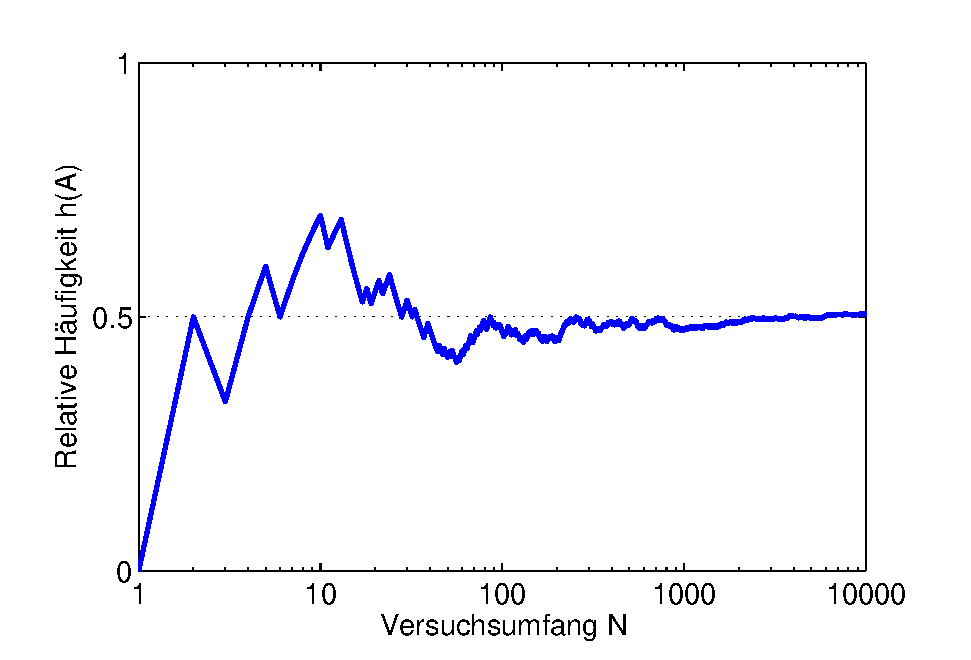
\includegraphics[width=0.7\textwidth]{Kapitel7/Bilder/image9}}
  \caption{Kunststoffgehäuse eines Luftmassenmessers der Robert Bosch GmbH [BOSC11]}
  \label{fig:Kunststoffgehäuse}
\end{figure}

\noindent Die Werkzeugma{\ss}e m\"{u}ssen so ausgelegt werden, dass Formteile mit den gew\"{u}nschten sp\"{a}teren Endma{\ss}en gefertigt werden k\"{o}nnen. Dabei muss die Schwindung des Bauteils ber\"{u}cksichtigt werden. Die Schwindung ist zwar in erster Linie eine Werkstoffeigenschaft, sie wird dar\"{u}ber hinaus aber auch bestimmt durch die Gestalt und Wanddicke des Spritzgussteils sowie durch die Verarbeitungsbedingungen. Das Zusammenwirken dieser verschiedenen Faktoren macht eine exakte Vorhersage der Schwindung meist sehr schwierig. Zur Ermittlung von praxisrelevanten Schwindungsma{\ss}en hat sich ein Testk\"{a}stchen bew\"{a}hrt, das in Bild \ref{fig:Testkörper} dargestellt ist. Ausgewertet wird meist die L\"{a}nge A als Ma{\ss} f\"{u}r die Schwindung des K\"{a}stchenbodens. [BASF11]

\noindent 
\begin{figure}[H]
  \centerline{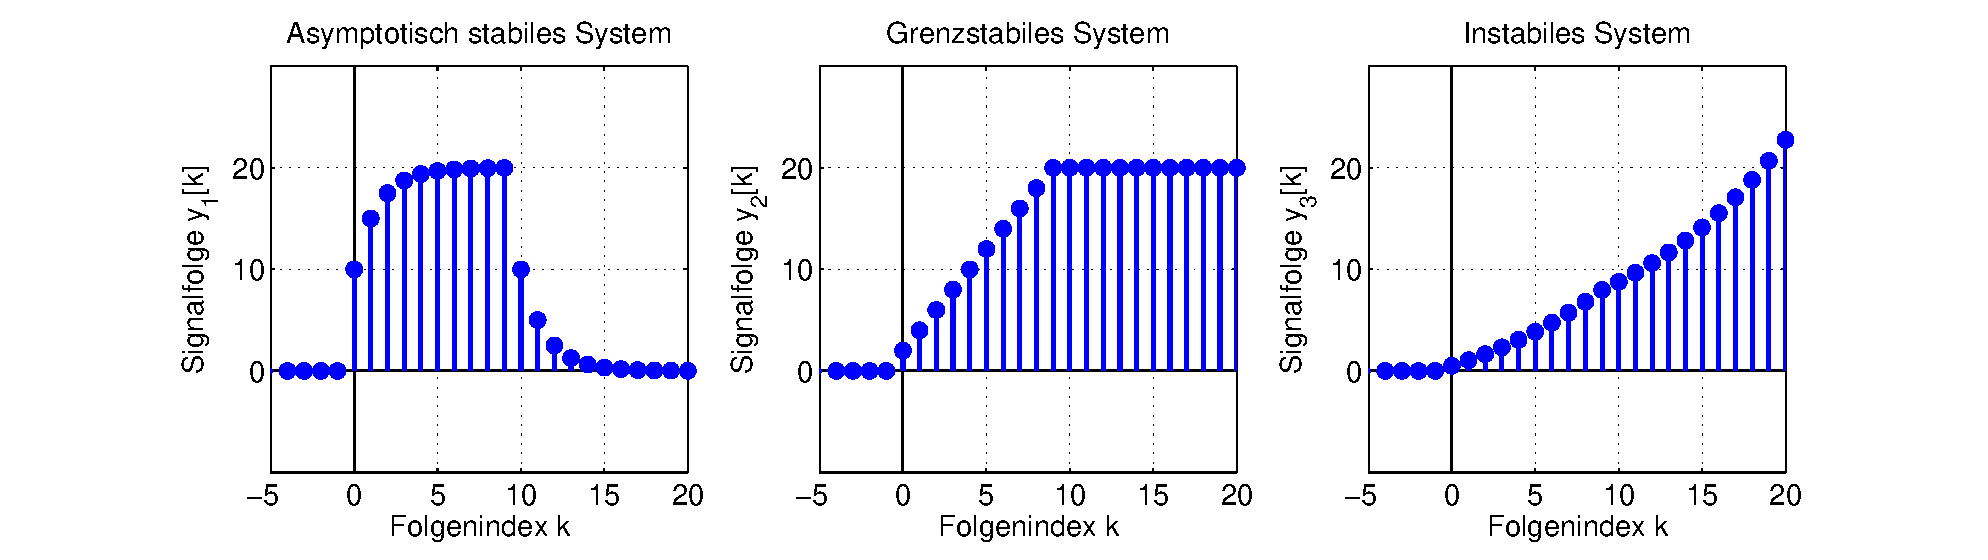
\includegraphics[width=0.5\textwidth]{Kapitel7/Bilder/image10}}
  \caption{Testkörper zur Ermittlung von praxisrelevanten Schwindungsma{\ss}en}
  \label{fig:Testkörper}
\end{figure}

\noindent Der Spritzgussprozess wird bei einer Werkzeugtemperatur T mit einem speziellen Druckprofil durchgef\"{u}hrt, das in Bild \ref{fig:Spritzgussprozess1} schematisch dargestellt ist. Die Einspritzung des geschmolzenen Kunststoffes erfolgt im Zeitraum von 0 {\dots} T$_{E}$ bei sehr hohen Dr\"{u}cken p$_{E}$. Ist das Spritzgusswerkzeug mit Kunststoff gef\"{u}llt, wird der Kunststoff f\"{u}r einen Zeitraum T$_{N}$ {\dots} T$_{A}$ einem definierten Nachdruck p$_{N}$ ausgesetzt. Anschlie{\ss}end wird der Kunststoff abgek\"{u}hlt und entformt. 

\noindent 
\begin{figure}[H]
  \centerline{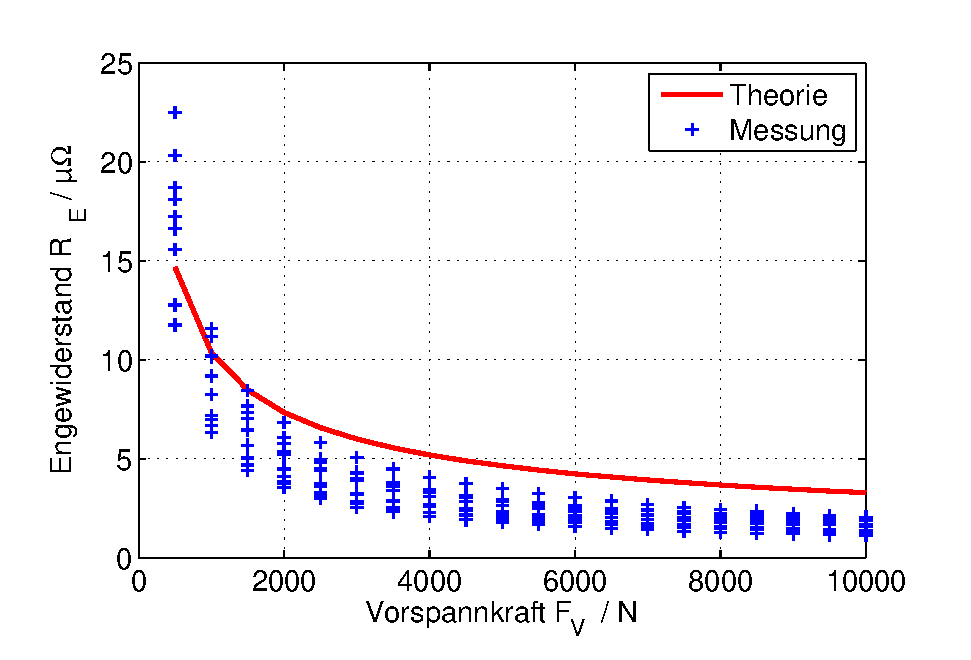
\includegraphics[width=0.5\textwidth]{Kapitel7/Bilder/image11}}
  \caption{Schematisierter Druckverlauf w\"{a}hrend eines Spritzgussvorgangs}
  \label{fig:Spritzgussprozess1}
\end{figure}

\noindent In einem Versuch wird die Schwindung des Bauteils unter unterschiedlichen Randbedingungen analysiert. Es ergibt sich der in Tabelle \ref{tab:seventwelve} dargestellte Datensatz.

\begin{table}[H]
\setlength{\arrayrulewidth}{.1em}
\caption{Urliste eines Versuchs zur Bewertung der Schwindung beim Spritzgie{\ss}en}
\setlength{\fboxsep}{0pt}%
\colorbox{lightgray}{%
\arrayrulecolor{white}%
\begin{tabular}{ wc{1.72cm} | wc{1.75cm} | wc{1.72cm} | wc{1.72cm} | wc{1.72cm} | wc{1.75cm} | wc{1.72cm} | wc{1.72cm}}
\hline\xrowht{10pt}

\fontfamily{phv}\selectfont\textbf{Wand-} &
\fontfamily{phv}\selectfont\textbf{Werkzeug-} &
\fontfamily{phv}\selectfont\textbf{Nach-} &
\fontfamily{phv}\selectfont\textbf{Schwin-} &
\fontfamily{phv}\selectfont\textbf{Wand-} &
\fontfamily{phv}\selectfont\textbf{Werkzeug-} &
\fontfamily{phv}\selectfont\textbf{Nach-} &
\fontfamily{phv}\selectfont\textbf{Schwin-} \\ 

\fontfamily{phv}\selectfont\textbf{dicke} &
\fontfamily{phv}\selectfont\textbf{temperatur} &
\fontfamily{phv}\selectfont\textbf{druck} &
\fontfamily{phv}\selectfont\textbf{dung} &
\fontfamily{phv}\selectfont\textbf{dicke} &
\fontfamily{phv}\selectfont\textbf{temperatur} &
\fontfamily{phv}\selectfont\textbf{druck} &
\fontfamily{phv}\selectfont\textbf{dung}\\

\fontfamily{phv}\selectfont\textbf{D / mm} &
\fontfamily{phv}\selectfont\textbf{T / $\si{\degree}$C} &
\fontfamily{phv}\selectfont\textbf{p$_{N}$ / bar} &
\fontfamily{phv}\selectfont\textbf{S / \%} &
\fontfamily{phv}\selectfont\textbf{D / mm} &
\fontfamily{phv}\selectfont\textbf{T / $\si{\degree}$C} &
\fontfamily{phv}\selectfont\textbf{p$_{N}$ / bar} &
\fontfamily{phv}\selectfont\textbf{S / \%}\\ \hline \xrowht{10pt}

\fontfamily{phv}\selectfont{1.5} &
\fontfamily{phv}\selectfont{31.2} &
\fontfamily{phv}\selectfont{508.0} &
\fontfamily{phv}\selectfont{1.20} &
\fontfamily{phv}\selectfont{8} &
\fontfamily{phv}\selectfont{60.1} &
\fontfamily{phv}\selectfont{740.5} &
\fontfamily{phv}\selectfont{2.39}\\ \hline \xrowht{10pt}

\fontfamily{phv}\selectfont{5} &
\fontfamily{phv}\selectfont{28.7} &
\fontfamily{phv}\selectfont{509.4} &
\fontfamily{phv}\selectfont{1.83} &
\fontfamily{phv}\selectfont{1.5} &
\fontfamily{phv}\selectfont{91.4} &
\fontfamily{phv}\selectfont{757.8} &
\fontfamily{phv}\selectfont{1.42}\\ \hline \xrowht{10pt}

\fontfamily{phv}\selectfont{8} &
\fontfamily{phv}\selectfont{30.8} &
\fontfamily{phv}\selectfont{490.1} &
\fontfamily{phv}\selectfont{2.42} &
\fontfamily{phv}\selectfont{5} &
\fontfamily{phv}\selectfont{91.1} &
\fontfamily{phv}\selectfont{755.7} &
\fontfamily{phv}\selectfont{2.07}\\ \hline \xrowht{10pt}

\fontfamily{phv}\selectfont{1.5} &
\fontfamily{phv}\selectfont{58.0} &
\fontfamily{phv}\selectfont{502.1} &
\fontfamily{phv}\selectfont{1.42} &
\fontfamily{phv}\selectfont{8} &
\fontfamily{phv}\selectfont{89.5} &
\fontfamily{phv}\selectfont{741.8} &
\fontfamily{phv}\selectfont{2.62}\\ \hline \xrowht{10pt}

\fontfamily{phv}\selectfont{5} &
\fontfamily{phv}\selectfont{60.0} &
\fontfamily{phv}\selectfont{502.4} &
\fontfamily{phv}\selectfont{2.08} &
\fontfamily{phv}\selectfont{1.5} &
\fontfamily{phv}\selectfont{29.2} &
\fontfamily{phv}\selectfont{997.3} &
\fontfamily{phv}\selectfont{0.70}\\ \hline \xrowht{10pt}

\fontfamily{phv}\selectfont{8} &
\fontfamily{phv}\selectfont{59.9} &
\fontfamily{phv}\selectfont{489.9} &
\fontfamily{phv}\selectfont{2.64} &
\fontfamily{phv}\selectfont{5} &
\fontfamily{phv}\selectfont{29.4} &
\fontfamily{phv}\selectfont{988.1} &
\fontfamily{phv}\selectfont{1.35}\\ \hline \xrowht{10pt}

\fontfamily{phv}\selectfont{1.5} &
\fontfamily{phv}\selectfont{90.0} &
\fontfamily{phv}\selectfont{492.6} &
\fontfamily{phv}\selectfont{1.67} &
\fontfamily{phv}\selectfont{8} &
\fontfamily{phv}\selectfont{27.0} &
\fontfamily{phv}\selectfont{978.0} &
\fontfamily{phv}\selectfont{1.90}\\ \hline \xrowht{10pt}

\fontfamily{phv}\selectfont{5} &
\fontfamily{phv}\selectfont{89.4} &
\fontfamily{phv}\selectfont{510.8} &
\fontfamily{phv}\selectfont{2.30} &
\fontfamily{phv}\selectfont{1.5} &
\fontfamily{phv}\selectfont{59.5} &
\fontfamily{phv}\selectfont{1009.9} &
\fontfamily{phv}\selectfont{0.92}\\ \hline \xrowht{10pt}

\fontfamily{phv}\selectfont{8} &
\fontfamily{phv}\selectfont{92.2} &
\fontfamily{phv}\selectfont{498.7} &
\fontfamily{phv}\selectfont{2.89} &
\fontfamily{phv}\selectfont{5} &
\fontfamily{phv}\selectfont{60.2} &
\fontfamily{phv}\selectfont{994.8} &
\fontfamily{phv}\selectfont{1.59}\\ \hline \xrowht{10pt}

\fontfamily{phv}\selectfont{1.5} &
\fontfamily{phv}\selectfont{26.3} &
\fontfamily{phv}\selectfont{753.9} &
\fontfamily{phv}\selectfont{0.92} &
\fontfamily{phv}\selectfont{8} &
\fontfamily{phv}\selectfont{60.6} &
\fontfamily{phv}\selectfont{1003.3} &
\fontfamily{phv}\selectfont{2.13}\\ \hline \xrowht{10pt}

\fontfamily{phv}\selectfont{5} &
\fontfamily{phv}\selectfont{30.9} &
\fontfamily{phv}\selectfont{750.9} &
\fontfamily{phv}\selectfont{1.60} &
\fontfamily{phv}\selectfont{1.5} &
\fontfamily{phv}\selectfont{92.9} &
\fontfamily{phv}\selectfont{1002.3} &
\fontfamily{phv}\selectfont{1.19}\\ \hline \xrowht{10pt}

\fontfamily{phv}\selectfont{8} &
\fontfamily{phv}\selectfont{31.8} &
\fontfamily{phv}\selectfont{743.6} &
\fontfamily{phv}\selectfont{2.17} &
\fontfamily{phv}\selectfont{5} &
\fontfamily{phv}\selectfont{89.3} &
\fontfamily{phv}\selectfont{1000.2} &
\fontfamily{phv}\selectfont{1.81}\\ \hline \xrowht{10pt}

\fontfamily{phv}\selectfont{1.5} &
\fontfamily{phv}\selectfont{61.5} &
\fontfamily{phv}\selectfont{744.4} &
\fontfamily{phv}\selectfont{1.20} &
\fontfamily{phv}\selectfont{8} &
\fontfamily{phv}\selectfont{91.2} &
\fontfamily{phv}\selectfont{990.0} &
\fontfamily{phv}\selectfont{2.39}\\ \hline \xrowht{10pt}

\fontfamily{phv}\selectfont{5} &
\fontfamily{phv}\selectfont{61.2} &
\fontfamily{phv}\selectfont{754.4} &
\fontfamily{phv}\selectfont{1.83} &
\fontfamily{phv}\selectfont{ } &
\fontfamily{phv}\selectfont{ } &
\fontfamily{phv}\selectfont{ } &
\fontfamily{phv}\selectfont{ }\\ \hline 

\end{tabular}%
}
\label{tab:seventwelve}
\end{table}

\noindent Um Abh\"{a}ngigkeiten der mehrdimensionalen Stichprobe eindeutig erkennen zu k\"{o}nnen, wird sie in einer Streudiagramm-Matrix dargestellt. Bild \ref{fig:Spritzgussprozess2} stellt die Streudiagramm-Matrix zur Urliste aus Tabelle \ref{tab:seventwelve} dar. Die Matrix ist symmetrisch zur Hauptdiagonalen. An der grafischen Darstellung kann abgelesen werden, welche Kombinationen von Dicke D, Temperatur T und Nachdruck p$_{N}$ zur Untersuchung der Schwindung verwendet wurden. Es wird au{\ss}erdem deutlich, dass die Schwindung ma{\ss}geblich von der Wanddicke D abh\"{a}ngig ist.

\noindent 
\begin{figure}[H]
  \centerline{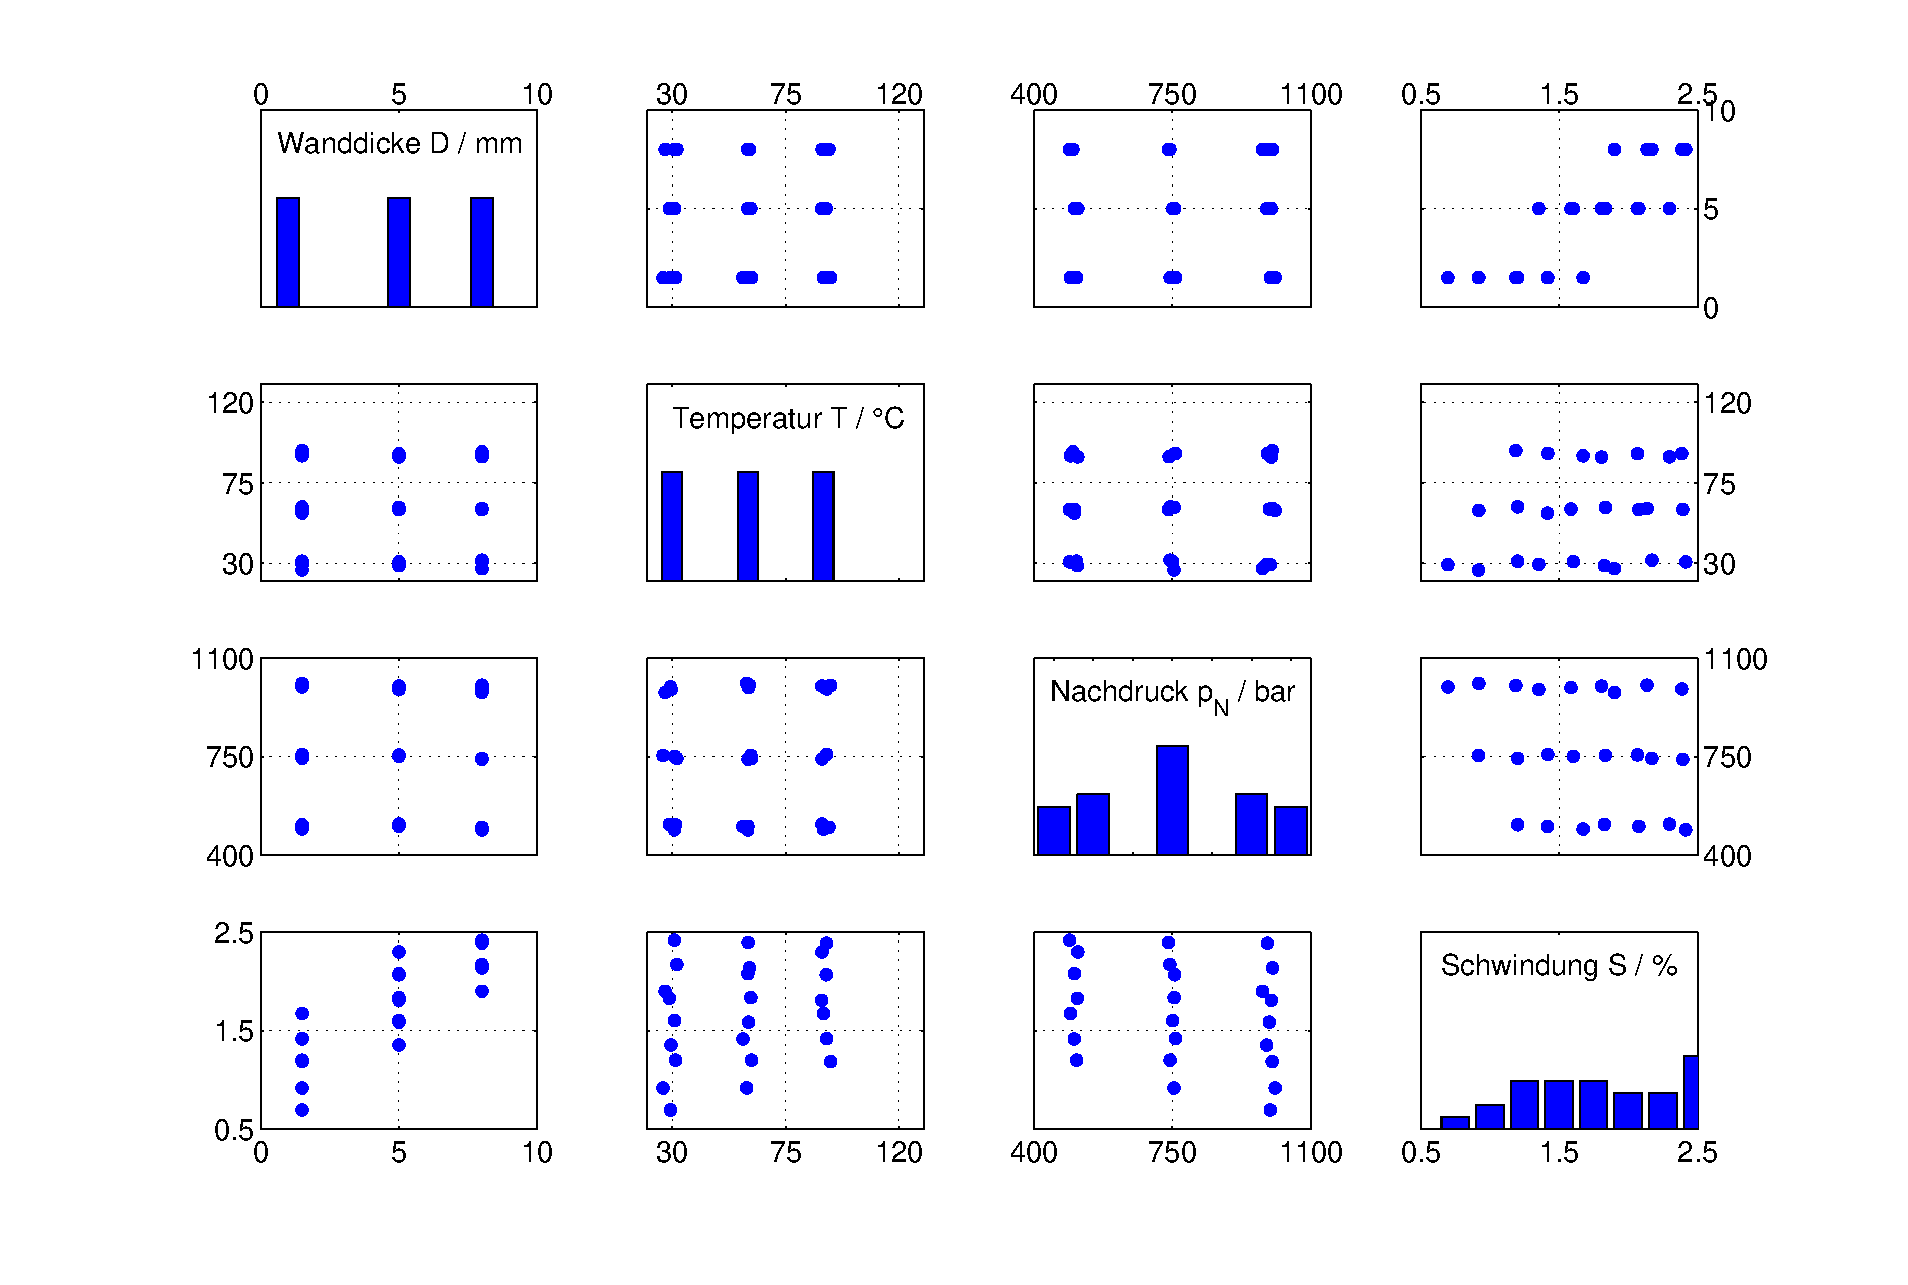
\includegraphics[width=1\textwidth]{Kapitel7/Bilder/image12}}
  \caption{Berechnung der Kennwerte der multivariaten Stichprobe aus Tabelle \ref{tab:seventwelve} erfolgt mit MATLAB durch}
  \label{fig:Spritzgussprozess2}
\end{figure}

\lstinputlisting[caption = {}]{Kapitel7/mat7.m}

\noindent Es ergibt sich ein Vektor der Mittelwerte von

\begin{equation}\label{eq:seventwentyeight}
\underline{\bar{x}}=\left(\begin{array}{cccc} {4.8333} & {60.1222} & {748.5519} & {1.8019} \end{array}\right)
\end{equation}

\noindent Die Kovarianzmatrix \textbf{S} berechnet sich zu

\begin{equation}\label{eq:seventwentynine}
S=\left(\begin{array}{cccc} {7.3269} & {0.3788} & {-11.2641} & {1.3661} \\ 
{0.3788} & {652.3241} & {28.1773} & {5.1260} \\
{-11.2641} & {28.1773} & {42564} & {-44.4499} \\ 
{1.3661} & {5.1260} & {-44.4499} & {0.3365} \end{array}\right)
\end{equation}

\noindent Die Daten der Kovarianzmatrix lassen sich wegen einer fehlenden Normierung nur bedingt interpretieren. Zum Beispiel ist die Varianz des Druckes aufgrund der hohen Zahlenwerte sehr hoch, auch die mit dem Druck verbundenen Kovarianzen haben vergleichsweise gro{\ss}e Werte. Deshalb wird zus\"{a}tzlich die Korrelationsmatrix \textbf{R} berechnet.

\begin{equation}\label{eq:seventhirty}
R=\left(\begin{array}{cccc} {1} & {0.0055} & {-0.0202} & {0.8700} \\ 
{0.0055} & {1} & {0.0053} & {0.3460} \\ 
{-0.0202} & {0.0053} & {1} & {-0.3714} \\ 
{0.8700} & {0.3460} & {-0.3714} & {1} \end{array}\right)
\end{equation}

\noindent Die gr\"{o}{\ss}te Korrelation zur Schwindung hat die Wandst\"{a}rke D. Wegen des positiven Vorzeichens stiegt die Schwindung mit steigender Wandst\"{a}rke. Im Gegensatz dazu liegt zwischen Nachdruck und Schwindung eine negative Korrelation vor, mit steigendem Nachdruck nimmt die Schwindung ab.\newline

\noindent Uneinheitliche Schwindung an unterschiedlichen Orten im Bauteil f\"{u}hrt dazu, dass sich ein Spritzgussteil verzieht. Um den Verzug im Bauteil zu verringern, muss bei der Konstruktion darauf geachtet werden, dass alle Teile eine vergleichbare Wandst\"{a}rke aufweisen.\newline

\noindent Erg\"{a}nzend ist unten ein Python-Beispiel zur Auswertung der Stichprobe aufgef\"{u}hrt.

\lstinputlisting[caption = {}]{Kapitel7/mat8.m}

\subsection{Literatur}

\begin{tabular}{|p{0.6in}|p{5.6in}|} \hline 
[Krey91] & Kreyszig, Erwin: Statistische Methoden und ihre Anwendungen\newline 4., unver\"{a}nderter Nachdruck der 7. Auflage\newline Vandenhoeck \& Ruprecht, G\"{o}ttingen, 1991 \\ \hline 
[Fahr96] & Fahrmeir, Ludwig; Hamerle, Alfred; Tutz, Gerhard: Multivariate statistische Verfahren\newline 2., \"{u}berarbeitete Auflage\newline Walter de Gryter \& Co., Berlin \\ \hline 
[Ross06] & Ross, M. Sheldon: Statistik f\"{u}r Ingenieure und Naturwissenschaftler\newline 3. Auflage\newline Spektrum Akademischer Verlag, M\"{u}nchen, 2006 \\ \hline 
[Hart07] & Hartung, Joachim; Elpelt, B\"{a}rbel: Multivariate Statistik\newline 7., unver\"{a}nderte Auflage\newline R. Oldenbourg Verlag, M\"{u}nchen / Wien \\ \hline 
[Papu01] & Papula, Lothar: Mathematik f\"{u}r Ingenieure und Naturwissenschaftler Band 3\newline 4., verbesserte Auflage\newline Vieweg Teubner, Braunschweig / Wiesbaden, 2008 \\ \hline 
[Wiki11] & Wikipedia: Spritzgie{\ss}enhttp://de.wikipedia.org , 22.04.2011 \\ \hline 
[BASF11] & BASF: Verpackungsportalhttp://www.packaging.basf.com, 22.04.2011 \\ \hline 
[BOSC11] & Robert Bosch GmbH: Hei{\ss}filmluftmassenmesser HFM7,Stuttgart, 2011 \\ \hline 
\end{tabular}

